\documentclass{article}

\usepackage{amsmath}
\usepackage{color}
\usepackage{amssymb}
\usepackage[english]{babel}
\usepackage{graphicx}
\usepackage{listings, multicol}
\usepackage{subfig}
\usepackage{tikz}
\usepackage{hyperref}
\usepackage{makeidx}
\usepackage{bm}
\usepackage{threeparttable}
\usepackage{array}
\usepackage{tabularx}
\usepackage{microtype}
\usepackage[htt]{hyphenat}
\usepackage{subfig}


\renewcommand{\arraystretch}{2}

\newcommand{\norm}[1]{\lVert#1\rVert}
\newcommand{\vect}[1]{\mathbf{#1}}
\newcommand{\bol}[1]{\boldsymbol{#1}}
\newcommand{\HiFlow}{HiFlow\texorpdfstring{\textsuperscript{3} }{3 }}
\definecolor{lbcolor}{rgb}{0.97,0.97,0.97}

%% Information for PDF-Datei
\hypersetup{
pdfauthor={Michael Schick},
pdftitle={Tutorial: Poisson equation with uncertain diffusivity parameter},
pdfsubject={Poisson Equation},
pdfkeywords={uncertainty quantification, polynomial chaos}
}

% Print URLs not in Typewriter Font
\def\UrlFont{\rm}

% Index-Datei öffnen
\makeindex
%%%%%%%%%%%%%%%%%%%%%%%%%%%%%%%%%%%%%%%%%%%%%%
\begin{document}

%Title page
\pagenumbering{roman}
\begin{titlepage}
\def\usesf{}
\let\usesf\sffamily % diese Zeile auskommentieren für normalen TeX Font
\setlength{\unitlength}{1pt}
\Large\bfseries \textsf{\hspace{30pt}Tutorial}
\thispagestyle{empty}\\ 
\noindent\rule{\textwidth}{1pt}
\begin{picture}(0,0)(-250,-25)

\includegraphics[scale=.22]{emcl.pdf} 
\end{picture}

\begin{center}
\hbox{}

{\usesf
\vspace{40pt}
{\normalsize\mdseries M. Schick, C. Song\\}
\vspace{20pt}
{\huge\bfseries Solving the Poisson equation with uncertain parameters using the Spectral-Stochastic-Finite-Element-Method\par}
\vspace{20pt}
{\normalsize\mdseries April 16$^\text{th}$, 2015\\}
\vskip 2.5cm


\includegraphics[scale=.4]{HF3_color.png} 

\vspace{-20pt}
\normalsize\mdseries{\hspace{170pt}Version 1.5}
}
\end{center}
\vfill
\noindent\rule{\textwidth}{1pt}
\begin{flushright}
\normalsize\mdseries\textsf{http://www.hiflow3.org\hspace{20pt}}
\end{flushright}
\end{titlepage}

% Contents
\renewcommand{\contentsname}{Contents}
\pagenumbering{Roman}

{\parskip 0pt\tableofcontents} % toc bitte einzeilig



%% ++++++++++++++++++++++++++++++++++++++++++
%% Main part
%% ++++++++++++++++++++++++++++++++++++++++++
\graphicspath{{Bilder/}}

\pagenumbering{arabic}
\renewcommand{\contentsname}{Introduction}

\pagebreak

\fbox{
\begin{minipage}{0.9\linewidth}\vspace*{15pt}\hspace*{15pt}\Large\textbf{Using HiFlow$^\textbf{3}$ for solving the\\\hspace*{15pt}Poisson equation with uncertain \\\hspace*{15pt}parameters}\vspace*{15pt}
\end{minipage}
}

\section{Introduction}

HiFlow$^\text{3}$ is a multi-purpose finite element software providing powerful tools for efficient and accurate solution of a wide range of problems modeled by partial differential equations (PDEs). Based on object-oriented concepts and the full capabilities of C++ the HiFlow$^\text{3}$  project follows a modular and generic approach for building efficient parallel numerical solvers. It provides highly capable modules dealing with the mesh setup, finite element spaces, degrees of freedom, linear algebra routines, numerical solvers, and output data for visualization. Parallelism - as the basis for high performance simulations on modern computing systems - is introduced on two levels: coarse-grained parallelism by means of distributed grids and distributed data structures, and fine-grained parallelism by means of platform-optimized linear algebra back-ends.

\subsection{How to use the Tutorial}

You find the example code (\texttt{poisson\_uncertainty.cc}, \texttt{poisson\_uncertainty.h}), a
parameter file (\texttt{poisson\_uncertainty/poisson\_uncertainty.xml})\index{configuration file}. The geometry data (\texttt{*.inp}) is stored in the
folder \texttt{/hiflow/examples/data/}.\index{geometry!folder}

\subsubsection{Using \HiFlow as a Developer}

First build and compile  HiFlow$^\text{3}$. Go to the directory \path{/build/examples/poisson_uncertainty}, where the binary poisson uncertainty tutorial is stored. Type \textbf{./poisson\_uncertainty poisson\_uncertainty.xml} to execute the program in sequential mode,  To execute in parallel mode with four processes for spatial decomposition and two processes for stochastic modes, type \textbf{mpirun -np 8 ./poisson\_uncertainty poisson\_uncertainty.xml 4 }. In both cases,you need to make sure that the default parameter file \texttt{poisson\_uncertainty.xml} is stored in the same directory as the binary, and that the geometry data specified in the parameter file is stored in \texttt{/hiflow/examples/data}. Alternatively, you can specify the path of your own xml-file with the name of your xml-file in the comment line, i.e. \textbf{mpirun -np 8 ./poisson\_uncertainty "path\_to\_parameterfile/name\_of\_parameterfile".xml 4}.

\pagebreak

\section{Mathematical Setup}
\label{sec:mathSetup}

\subsection{Problem}

We consider the Poisson equation with uncertain, spatially dependent diffusivity parameter $\nu$. The equations are imposed on the unit-square, i.e., $\Omega = [0,1]^2$. The boundary conditions and the forcing term are assumed to be deterministic.

The governing equations can be expressed by :

\begin{align}
\label{eq:poisson_init1}
-\nabla \cdot (\nu(x, \theta) \nabla u(x, \theta)) &= 1, &x \in \Omega, \theta \in \Theta \\
\label{eq:poisson_init2}
u(x, \theta) &= 1, &x \in \Gamma, \theta \in \Theta \\
\label{eq:poisson_init3}
\dfrac{\partial u}{\partial x} (x, \theta) &= 0, &x \in \partial \Omega \backslash \Gamma, \theta \in \Theta
\end{align}

Here, the Dirichlet boundary $\Gamma$ is defined as $\Gamma = \{ x = (x_{1}, 0) \in \Omega, x_1 \in [0,1] \} $.  $\Theta$ denotes the abstract sampling space of the uncertain event $\theta \in \Theta$. We introduce an uncertainty model for $\nu(x,\theta)$ by:

\begin{align}
\label{eq:uncertain}
\nu(x,\theta) &= \nu_0 + \nu_0 \sigma \sum_{i=1}^M q^{i-1}\sin(2\pi ix_1)\sin(2\pi ix_2)\xi_i(\theta),
\end{align}

where $\bm{\xi(\theta)} := (\xi_1(\theta),\ldots,\xi_M(\theta))$ denotes a random vector, components of which are independent and uniformly distributed in the interval $[-1,1]$, i.e., $\xi_i \sim \mathcal{U}(-1,1)$. The mean of $\nu(x,\theta)$ is then $\mathbb{E}(\nu) = \nu_0$ by definition. The stochastic parameter $\sigma$ denotes the magnitude of fluctuation of the diffusivity around its mean. The parameter $q$ denotes the decay rate of the fluctuations. In order to obtain a well-posed problem, we need to enforce that :

\begin{equation*}
0 < q < 1,\quad\text{and } 0 < \dfrac{\sigma}{1-q} < 1.
\end{equation*}
The notation of $\theta$ will be dropped in the following equations, due to the fact that we consider only the uncertain parameter vector \bm{$\xi$} in our mathematical set-up. In general, the governing PDE could be carried out from \eqref{eq:poisson_init1} - \eqref{eq:poisson_init3} with $\xi$:

\begin{align}
\label{eq:poisson}
-\nabla \cdot (\nu(x, \bm{\xi}) \nabla u(x, \bm{\xi})) &= 1, &&x \in \Omega, \\
u(x, \bm{\xi}) &= 1, &&x \in \Gamma, \\
\dfrac{\partial u}{\partial x}(x, \bm{\xi}) &= 0, &&x \in \partial \Omega \backslash \Gamma
\end{align}

where the equations are required to hold almost surely in $\Theta$.

\subsection{Using Polynomial Chaos as a basis for stochastic part}

We assume a square-integrable stochastic solution, i.e., $u(x,\cdot) \in L^2(\Xi)$ for all $x \in [0,1]^2$ with $\Xi$ denoting the range of $\bm{\xi}$. Then we can express the stochastic solution using a spectral expansion:

\begin{equation}
\label{eq:spectral}
u(x, \bm{\xi}) = \sum_{i=0}^{+\infty} u_{i}(x) \psi_{i}(\bm{\xi}),
\end{equation}

where, $u_{i}(x)$ denotes the \textbf{deterministic part}, and $\psi_{i}(\bm{\xi})$ denotes the \textbf{stochastic part}. We use the Polynomial Chaos (PC) expansion for choosing the basis functionals $\psi_{i}(\bm{\xi})$. In standard formulation, these correspond to multivariate Hermite-Polynomials in terms of Gaussian random variables \cite{wiener1938}. However, since we assume a Uniform distribution for \bm{$\xi$} we use multivariate Legendre Polynomials instead, since these satisfy an orthogonality condition with respect to the constant probability density function $1/2^M$ of \bm{$\xi$}:

\begin{align*}
\langle\psi_{n},\psi_{m}\rangle &:= \dfrac{1}{2^M}\int_{[-1,1]^M} \psi_{n}(\bm{\xi}) \psi_{m}(\bm{\xi}) d\bm{\xi} = \|\psi_n\|_{L^2(\Xi)}^2 \delta_{n,m} \\
\mathbb{E}[\psi_{0}] &= \dfrac{1}{2^M}\int_{[-1,1]^M} \psi_{0}(\bm{\xi}) d\bm{\xi} = 1 \\
\mathbb{E}[\psi_{n}] &= \dfrac{1}{2^M}\int_{[-1,1]^M} \psi_{n}(\bm{\xi}) d\bm{\xi} = 0, n > 0
\end{align*}

The multivariate Chaos Polynomials can be computed by a tensor product of their one-dimensional counterpart, see for example \cite{Xiu:2002:WPC:587159.587325}.

The expectation $\mathbb{E}$ and the variance $\sigma^2$ of the \textbf{stochastic solution} $u(x,\xi)$ can be computed by:

\begin{align}
\mathbb{E}[u](x) &= \dfrac{1}{2^M}\int_{[-1,1]^M} \sum_{i=0}^{+\infty} u_{i}(x) \psi_{i} d\xi = u_{0}(x) \\
\sigma^2[u](x) &= \mathbb{E}[u^{2}](x) - (\mathbb{E}[u](x))^{2} = \sum_{i=1}^{+\infty} u_{i}^{2}(x) \langle\psi_{i},\psi_i\rangle.
\end{align}

In order to achieve a finite-dimensional approximation for numerical computation, we need to truncate the stochastic spectral expansion \eqref{eq:spectral}. We do so by prescribing a maximum total polynomial degree $p$ for the polynomials $\{\psi_i\}$, such that

\begin{equation}
\label{eq:truncated_poly_multi}
u(x,\bm{\xi}) = \sum_{i=0}^{P} u_i(x) \psi_{i}(\bm{\xi}),
\end{equation}
where the number of terms $P+1$ are given by \cite{maitre2010spectral}
\begin{equation}
\label{eq:modes}
P+1 = \dfrac{(p+M)!}{p!M!}.
\end{equation}

Currently, two distributions are implemented in HiFlow$^3$, which are stated in Table \ref{tab:polynomials}.

\begin{table}[hbtp]\small
	\centering
	\begin{tabular}{|c|c|c|c|}
	\cline{1-4}
	\textbf{Distribution} & \textbf{pdf} & \textbf{Polynomials}  & \textbf{Support} \\ \cline{1-4}
	Uniform & $\frac{1}{2}$ & Legendre & $[-1,1]$ \\ \cline{1-4}
	Gaussian & $\frac{e^{-x^{2}/2}}{\sqrt{2 \pi}}$ & Hermite & $[-\infty, + \infty]$ \\ \cline{1-4} 
	\end{tabular}
	\begin{tablenotes}
	\item[*] pdf: probability density functions
	\end{tablenotes}
	\caption{Chaos Polynomials implemented in HiFlow$^3$.}
	\label{tab:polynomials}
\end{table}


\subsection{Discretization by stochastic Galerkin projection}
We introduce a short notation for the stochastic diffusivity parameter $\nu = \nu(x,\bm\xi)$ for notational convenience:
\begin{equation}
\label{eq:nu-short}
\nu(x,\bm\xi) = \sum_{i=0}^M \nu_i(x)\psi_i(\bm\xi),
\end{equation}
where
\begin{align*}
\nu_0(x) &:= \nu_0,\\
\nu_i(x) &:= \nu_0\sigma q^{i-1}\sin(2\pi i x_1)\sin(2\pi i x_2), \quad i=1,\ldots,M.
\end{align*}
Note, that by definition of the Chaos Polynomials, we have
\begin{equation}
\psi_i(\bm\xi) = \xi_i,\quad i=1,\ldots,M.
\end{equation}
We illustrate the stochastic Galerkin approach on \eqref{eq:poisson}. The boundary conditions can be discretized in a similar way. The stochastic Galerkin projection is based on a variational setting of \eqref{eq:poisson} with respect to the stochastic space $L^2(\Xi)$. By $\mathcal{S}_p \subset L^2(\Xi)$ we denote the space spanned by the Chaos Polynomials up to total degree $p$, i.e., $\mathcal{S}_p = span\{\psi_0,\psi_1,\ldots,\psi_P\}$.

The corresponding (discrete) variational setting with respect to the stochastic space reads: find $u(x,\cdot) \in \mathcal{S}_p$ such that
\begin{equation}
\label{eq:poisson-variational}
-\langle \nabla\cdot(\nu(x,\bm\xi)\nabla u(x,\bm\xi)),\psi \rangle = \langle 1,\psi \rangle,\quad \forall \psi \in \mathcal{S}_p.
\end{equation}
for all $x \in [0,1]^2$. Next we insert \eqref{eq:nu-short} and \eqref{eq:truncated_poly_multi} into \eqref{eq:poisson-variational} and get by orthogonality of the Chaos Polynomials
\begin{equation}
\label{eq:stochastic-galerkin}
-\sum_{i=0}^M\sum_{j=0}^P \nabla\cdot(\nu_i(x)\nabla u_j(x)) c_{ijk} = \delta_{0,k},\quad \forall k=0,\ldots,P,
\end{equation}
where we define the third order stochastic Galerkin Tensor $\mathbb{T} = (c_{ijk})$ by \cite{maitre2010spectral}
\begin{equation}
c_{ijk} := \dfrac{\langle \psi_i\psi_j,\psi_k \rangle}{\langle \psi_k,\psi_k \rangle}.
\end{equation}
Finally, we obtained a deterministic set of coupled partial differential equations for the PC modes $u_i(x),\, i=0,\ldots,P$, which is solved using the Finite-Element-Method.

\subsection{Numerical methods for the solution of the linear systems}
The user of this tutorial can choose between two types of solution methods: CG (conjugate gradient) with or without mean-based preconditioning, and a stochastic multilevel solver, which is based on the hierarchical multilevel structure of the Chaos Polynomials
\begin{equation*}
\mathcal{S}_0 \subset \mathcal{S}_1 \subset \cdots \subset \mathcal{S}_p.
\end{equation*}
The mean-based preconditioner for CG is using an approximation of \eqref{eq:stochastic-galerkin} by means of a block-diagonal approach. Therefore, all terms $\nu_i(x)$ are set to zero for all $i > 0$, such that only the mean of $\nu$ is used in the preconditioning step. Therefore, due to orthogonality of the Chaos Polynomials $\psi_i$ the system simplifies to a single deterministic system (the so-called mean system). This is used for a preconditioning step for all $u_i(x)$ in order to speed up the convergence of CG. 

In the corresponding xml-file (see section \ref{sec:program:subsec:param_file}) with \texttt{<LinearSolver>}, this can be done by choosing either \texttt{CG} or \texttt{ML} for linear solver, and \texttt{Preconditioner} could also be modified with according preconditioner respectively.


\pagebreak
\section{The Commented Program}
\label{sec:program}


\subsection{Preliminaries}
\label{sec:program:subsec:prelim}

HiFLow$^\text{3}$ is designed for high performance computing on massively parallel machines. So it applies the Message Passing Interface (MPI) library specification for message-passing, see sections \ref{sec:program:subsec:main_func} and \ref{sec:program:subsec:member_func}, also \cite{MPI}. The poisson uncertainty tutorial needs the following two input files:

\begin{itemize}
\item \texttt{poisson\_uncertainty.xml}\index{configuration file} A xml-file containing all information needed to execute the program. It is read in by the program at runtime and thus does not require the recompilation of the program when parameters are changed. Parameters for example defining the termination condition of the linear solver and preconditioner are listed as well as parameters of polynomial degree and number of uncertain parameter. xml-file needs to be provided explicitly when poisson uncertainty executes, as it is described in section \ref{sec:intro:subsec:library}, the default xml-file is referred in section \ref{sec:program:subsec:param_file}, which contains the parameters of the two-dimensional numerical example, see section \ref{sec:example}. This file is stored in \texttt{/hiflow/examples/poisson\_uncertainty/}.

\item Geometry data\index{geometry!file}: The file containing the geometry is specified in the parameter file. In the example in section \ref{sec:example}, we used   \texttt{unit\_square.inp}
\end{itemize}

HiFlow$^\text{3}$ does not generate meshes for the domain $\Omega$. Meshes in \texttt{*.inp} and \texttt{*.vtu}\index{file format!inp} \index{file format!vtu} format can be read in. It is possible to extend the reader for other formats. Some geometry data is provided in the test/data folder. Furthermore it is possible to generate other geometries by using external programs (Mesh generators) or by hand. Both formats provide the possibility to mark cell or facets by material numbers.

\subsection{Parameter File}
\label{sec:program:subsec:param_file}

The needed parameters are initialized in the parameter file \texttt{poisson\_uncertainty.xml}.

\definecolor{gray}{rgb}{0.4,0.4,0.4}
\definecolor{darkblue}{rgb}{0.0,0.0,0.6}
\definecolor{cyan}{rgb}{0.2,0.6,0.7}

\lstset{
  basicstyle=\scriptsize,
  columns=fullflexible,
  showstringspaces=false,
  commentstyle=\color{gray}\upshape
}

\lstdefinelanguage{XML}
{
  morestring=[b]",
  morestring=[s]{>}{<},
  morecomment=[s]{<?}{?>},
  stringstyle=\color{black},
  identifierstyle=\color{cyan},
  keywordstyle=\color{darkblue},
  morekeywords={xmlns,version,type}% list your attributes here
}

\lstset{
  language=XML
}

\begin{lstlisting}
<Param>
  <Mesh>
    <Filename>unit_square.inp</Filename>
    <RefinementLevel>6</RefinementLevel>
<!--    <Filename>unit_cube.inp</Filename>-->
<!--    <RefinementLevel>4</RefinementLevel>-->
  </Mesh>
  <GalerkinLinearSolver>
    <LinearSolver>CG</LinearSolver>
<!--    <LinearSolver>Multilevel</LinearSolver>-->
<!--    <Preconditioner>None</Preconditioner>-->
<!--    <Preconditioner>Mean</Preconditioner>-->
    <Preconditioner>ML</Preconditioner>
  </GalerkinLinearSolver>
  <Multilevel>
    <MLType>Matrix</MLType>
    <Nu1>1</Nu1>
    <Nu2>1</Nu2>
    <Mu>1</Mu>
<!--    <Smoothing>Umfpack</Smoothing>-->
<!--    <Smoothing>InexactPCG</Smoothing>-->
    <Smoothing>InexactCG</Smoothing>
  </Multilevel>
  <Output>
    <InfoFilename>uq_poisson_mpi.info</InfoFilename>
    <MeshFilename>uq_poisson_mesh.vtu</MeshFilename>
    <VisuFolder>./</VisuFolder>
  </Output>
  <PolynomialChaos>
    <No>3</No>
    <N>6</N>
    <q>1</q>
  </PolynomialChaos>
  <Application>
    <MeanViscosity>0.01</MeanViscosity>
    <Variability>0.2</Variability>
    <Decay>0.5</Decay>
  </Application>
</Param>
\end{lstlisting}
\vspace{15pt}

\subsection{Main Function}
\label{sec:program:subsec:main_func}

The main function starts the simulation of the stochastic Poisson problem (\texttt{poisson\_uncertainty.cc}).

\lstset{
        language=[Visual]C++,
        keywordstyle=\ttfamily\color[rgb]{0,0,1},
        identifierstyle=\ttfamily,
        commentstyle=\color[rgb]{0.133,0.545,0.133},
        stringstyle=\ttfamily\color[rgb]{0.627,0.126,0.941},
        showstringspaces=false,
        basicstyle=\scriptsize,
%         numberstyle=\scriptsize,
%         numbers=left,
%         stepnumber=1,
%         numbersep=10pt,
        tabsize=2,
        breaklines=true,
        prebreak = \raisebox{0ex}[0ex][0ex]{\ensuremath{\hookleftarrow}},
        breakatwhitespace=false,
        aboveskip={1.5\baselineskip},
  columns=fixed,
  upquote=true,
  extendedchars=true,
frame=single,
% backgroundcolor=\color{lbcolor},
}
\begin{lstlisting}
.
int main ( int argc, char** argv )
{
    MPI_Init ( &argc, &argv );
    std::string fName;
    if ( argc > 1 )
    {
        fName = argv[1];
    }
    else
    {
        std::cout << "Pass XMl parameter file as argument!" << std::endl;
        std::cout << "Usage: ./poisson_uncertainty <xml-filename>" << std::endl;
        exit ( -1 );
    }

    // Setup timer.
    Timer main_timer;

    int num_partitions_space = 1;
    if ( argc > 2 )
        num_partitions_space = std::atoi ( argv[2] );
    // Read parameters
    PropertyTree config ( fName, MASTER_RANK, MPI_COMM_WORLD );

    // Start Logging
    std::ofstream info_file ( config["Output"]["InfoFilename"].get<std::string>( ).c_str ( ) );
    LogKeeper::get_log ( "info" ).set_target ( &info_file );
    // LogKeeper::get_log("info").set_target(&std::cout);
    int size;
    MPI_Comm_size ( MPI_COMM_WORLD, &size );
    LOG_INFO ( "MPI Processes", size );

    // Compute MPI subgroup for sequential domain treatment
    MPI_Comm comm_space;
    MPI_Comm comm_uq;

    MPI_Group orig_group, new_group_space, new_group_uq;
    MPI_Comm_group ( MPI_COMM_WORLD, &orig_group );

    int num_processors = size;
    int num_partitions_uq = num_processors / num_partitions_space;

    int my_rank;
    MPI_Comm_rank ( MPI_COMM_WORLD, &my_rank );

    int* ranks = new int[num_partitions_space];
    for ( int i = 0; i < num_partitions_space; ++i )
        ranks[i] = my_rank % num_partitions_uq + i * num_partitions_uq;

    MPI_Group_incl ( orig_group, num_partitions_space, ranks, &new_group_space );
    MPI_Comm_create ( MPI_COMM_WORLD, new_group_space, &comm_space );

    delete[] ranks;
    ranks = new int[num_partitions_uq];
    for ( int i = 0; i < num_partitions_uq; ++i )
        ranks[i] = my_rank - my_rank % num_partitions_uq + i;

    MPI_Group_incl ( orig_group, num_partitions_uq, ranks, &new_group_uq );
    MPI_Comm_create ( MPI_COMM_WORLD, new_group_uq, &comm_uq );
    delete[] ranks;

    // Run application
    PoissonMPI application ( config, comm_space, comm_uq );
    application.run ( );

    // flush log here to avoid problems
    LogKeeper::get_log ( "info" ).flush ( );

    // Stop timer.
    main_timer.stop ( );
    LOG_INFO ( "Total program run time [without MPI Init and Finalize]",
               main_timer );

    MPI_Finalize ( );
    return 0;
}
\end{lstlisting}

\subsection{Member Functions}
\label{sec:program:subsec:member_func}

Following member functions are components of the poisson uncertainty tutorial:

\begin{itemize}
\item{\texttt{run()}}
\item{\texttt{setup\_mesh()}}
\item{\texttt{setup\_application()}}
\item{\texttt{setup\_space()}}
\item{\texttt{setup\_system()}}
\item{\texttt{setup\_la\_structure()}}
\item{\texttt{setup\_linear\_solver()}}
\item{\texttt{setup\_bc()}}
\item{\texttt{setup\_linear\_system()}}
\item{\texttt{compute\_matrix()}}
\item{\texttt{compute\_residual()}}
\item{\texttt{visualize\_solution()}}
\end{itemize}


\subsubsection{run()}
\label{sec:program:subsec:run}

\lstset{
        language=[Visual]C++,
        keywordstyle=\ttfamily\color[rgb]{0,0,1},
        identifierstyle=\ttfamily,
        commentstyle=\color[rgb]{0.133,0.545,0.133},
        stringstyle=\ttfamily\color[rgb]{0.627,0.126,0.941},
        showstringspaces=false,
        basicstyle=\normalsize,
%         numberstyle=\scriptsize,
%         numbers=left,
%         stepnumber=1,
%         numbersep=10pt,
        tabsize=2,
        breaklines=true,
        prebreak = \raisebox{0ex}[0ex][0ex]{\ensuremath{\hookleftarrow}},
        breakatwhitespace=false,
        aboveskip={1.5\baselineskip},
  columns=fixed,
  upquote=true,
  extendedchars=true,
frame=single,
% backgroundcolor=\color{lbcolor},
}

The member function \texttt{run()} calls the functions \texttt{compute\_matrix()},  \texttt{compute\_residual()}, \texttt{setup\_linear\_solver()}, \texttt{solve\_linear\_system()} and \texttt{visualize\_solution()} to solve the stochastic Poisson problem which is described in section \ref{sec:mathSetup}. 

\lstset{
        language=[Visual]C++,
        keywordstyle=\ttfamily\color[rgb]{0,0,1},
        identifierstyle=\ttfamily,
        commentstyle=\color[rgb]{0.133,0.545,0.133},
        stringstyle=\ttfamily\color[rgb]{0.627,0.126,0.941},
        showstringspaces=false,
        basicstyle=\scriptsize,
%         numberstyle=\scriptsize,
%         numbers=left,
%         stepnumber=1,
%         numbersep=10pt,
        tabsize=2,
        breaklines=true,
        prebreak = \raisebox{0ex}[0ex][0ex]{\ensuremath{\hookleftarrow}},
        breakatwhitespace=false,
        aboveskip={1.5\baselineskip},
  columns=fixed,
  upquote=true,
  extendedchars=true,
frame=single,
% backgroundcolor=\color{lbcolor},
}

\begin{lstlisting}[firstnumber=39]
void PoissonMPI::run ( )
{
    compute_matrix ( );
    compute_residual ( );

    setup_linear_solver ( );

    Timer timer;
    timer.start ( );
    solve_linear_system ( );
    timer.stop ( );
    if ( pctensor_.MyRank ( ) == 0 )
        std::cout << "Solving linear system = " << timer.get_duration ( ) << "\n";

    std::string visu_folder = ( *config_ )["Output"]["VisuFolder"].get<std::string>( );

    for ( int mode = 0; mode < pctensor_.SizeLocal ( ); ++mode )
    {
        std::stringstream input;
        input << visu_folder;
        int glo_mode = pctensor_.L2G ( mode );
        input << "uq_poisson_mode_" << glo_mode;
        visualize_solution ( *galerkin_sol_->Mode ( mode ), input.str ( ) );
    }
}
\end{lstlisting}

\subsubsection{setup\_mesh()}

The member function \texttt{setup\_mesh()} reads in the mesh (\texttt{unit\_square.int})

\begin{lstlisting}
void PoissonMPI::setup_mesh ( )
{
    assert ( DIM == 2 || DIM == 3 );
    LOG_INFO ( "Problem dimension", DIM );
    ( *config_ )["Mesh"]["RefinementLevel"].read<int>( refinement_level_ );
    LOG_INFO ( "Refinement level", refinement_level_ );

    if ( rank_ == MASTER_RANK )
    {
        // read mesh (sequential, dimension DIM
        std::string mesh_filename = std::string ( DATADIR ) + ( *config_ )["Mesh"]["Filename"].get<std::string>( );
        master_mesh_ = read_mesh_from_file ( mesh_filename, DIM, DIM, 0 );

        for ( int r = 0; r < refinement_level_; ++r )
        {
            master_mesh_ = master_mesh_->refine ( );
        }
    }

    MeshPtr local_mesh = partition_and_distribute ( master_mesh_, MASTER_RANK, comm_space_ );
    assert ( local_mesh != 0 );
    SharedVertexTable shared_verts;
    mesh_ = compute_ghost_cells ( *local_mesh, comm_space_, shared_verts );

    std::ostringstream rank_str;
    rank_str << rank_;
    PVtkWriter writer ( comm_space_ );
    std::string output_file = ( *config_ )["Output"]["MeshFilename"].get<std::string>( );
    writer.write ( output_file.c_str ( ), *mesh_ );
}
\end{lstlisting}


\subsubsection{setup\_application()}

The member function \texttt{setup\_application()} sets the polynomial chaos information and computes the tensor structure.

\begin{lstlisting}
void PoissonMPI::setup_application ( )
{
    // setup stochastic parameters
    ( *config_ )["PolynomialChaos"]["No"].read<int>( No_ );
    LOG_INFO ( "Polynomial Chaos order", No_ );
    ( *config_ )["PolynomialChaos"]["N"].read<int>( N_ );
    LOG_INFO ( "Dimension of random space", N_ );
    // Polynomial degree of random input -> here: linear random input
    No_input_ = 1;
    LOG_INFO ( "Polynomial degree of random input", No_input_ );
    std::vector<PCBasis::Distribution> dist ( N_, PCBasis::UNIFORM );
    LOG_INFO ( "Probability distribution", "UNIFORM" );

    pcbasis_.Init ( N_, No_, dist );
    pctensor_.SetMPIComm ( comm_uq_ );
    pctensor_.ComputeTensor ( No_input_, pcbasis_ );

    double nu0, sigma, q;
    ( *config_ )["Application"]["MeanViscosity"].read<double>( nu0 );
    ( *config_ )["Application"]["Variability"].read<double>( sigma );
    ( *config_ )["Application"]["Decay"].read<double>( q );

    nu_.resize ( N_ + 1, 0.0 );
    nu_[0] = nu0;
    for ( int i = 1; i < N_ + 1; ++i )
        nu_[i] = sigma * nu0 * pow ( q, i - 1.0 );
}
\end{lstlisting}

\subsubsection{setup\_space()}

The member function \texttt{setup\_space()} sets vector space.

\begin{lstlisting}
void PoissonMPI::setup_space ( )
{
    // setup space Q1 elements
    space_ = new VectorSpace<double>( comm_space_ );
    int p_degree = 0;
    ( *config_ )["PolynomialChaos"]["q"].read<int>( p_degree );
    std::vector<int> degrees ( 1, p_degree );
    space_->Init ( degrees, *mesh_ );

    std::cout << "Rank: " << pctensor_.MyRank ( ) << " using NDofs = " <<
            space_->dof ( ).get_nb_dofs ( )*( pctensor_.SizeLocal ( ) + pctensor_.SizeOffModes ( ) ) << "\n";

    if ( pctensor_.MyRank ( ) == 0 )
        std::cout << "Number of Total Dofs: " << space_->dof ( ).get_nb_dofs ( ) << "x"
        << pctensor_.Size ( ) << " = " << ( long ) space_->dof ( ).get_nb_dofs ( ) * pctensor_.Size ( ) << "\n";
}
\end{lstlisting}


\subsubsection{setup\_system()}

The member function \texttt{setup\_system()} sets the computing platform.

\begin{lstlisting}
void PoissonMPI::setup_system ( )
{
    la_sys_.Platform = CPU;
    la_sys_.rank = 0;
    init_platform ( la_sys_ );
    matrix_impl_ = NAIVE;
    vector_impl_ = NAIVE;
    la_matrix_format_ = CSR;
    matrix_precond_ = NOPRECOND;
    la_sys_.GPU_CUBLAS = false;
}
\end{lstlisting}

\subsubsection{setup\_la\_structure()}

The member function \texttt{setup\_la\_structure()} sets the linear algebra structure.
 
\begin{lstlisting}
void PoissonMPI::setup_la_structures ( )
{
    // Initialize linear algebra structures
    couplings_.Clear ( );
    couplings_.Init ( comm_space_, space_->dof ( ) );

    // compute matrix graph to build matrix structure
    std::vector<int> diagonal_rows, diagonal_cols, off_diagonal_rows, off_diagonal_cols;
    std::vector < std::vector<bool> > var_coupling ( 1 );
    var_coupling[0].resize ( 1, true );
    InitStructure ( *space_, &diagonal_rows, &diagonal_cols,
                    &off_diagonal_rows, &off_diagonal_cols, &var_coupling );

    couplings_.InitializeCouplings ( off_diagonal_rows, off_diagonal_cols );

    // Initialize matrices and vectors
    matrix_.Init ( comm_space_, couplings_, la_sys_.Platform,
                   matrix_impl_, la_matrix_format_ );

    matrix_.InitStructure ( vec2ptr ( diagonal_rows ),
                            vec2ptr ( diagonal_cols ),
                            diagonal_rows.size ( ),
                            vec2ptr ( off_diagonal_rows ),
                            vec2ptr ( off_diagonal_cols ),
                            off_diagonal_rows.size ( ) );

    sol_.Init ( comm_space_, couplings_, la_sys_.Platform, vector_impl_ );
    sol_.InitStructure ( );
    sol_.Zeros ( );

    galerkin_matrix_.resize ( pcbasis_.N ( ) + 1 );
    for ( int i = 0; i < pcbasis_.N ( ) + 1; ++i )
        galerkin_matrix_[i] = new CoupledMatrix<double>;

    galerkin_sol_tmp_.resize ( pctensor_.SizeLocal ( ) + pctensor_.SizeOffModes ( ) );

    for ( int i = 0; i<static_cast < int > ( galerkin_sol_tmp_.size ( ) ); ++i )
    {
        galerkin_sol_tmp_[i] = new CoupledVector<double>;
        galerkin_sol_tmp_[i]->CloneFrom ( sol_ );
    }

    galerkin_sol_ = new PCGalerkinVector<double>;
    galerkin_res_ = new PCGalerkinVector<double>;
    galerkin_cor_ = new PCGalerkinVector<double>;

    galerkin_sol_->SetMPIComm ( comm_uq_ );
    galerkin_res_->SetMPIComm ( comm_uq_ );
    galerkin_cor_->SetMPIComm ( comm_uq_ );

    galerkin_sol_->SetModes ( galerkin_sol_tmp_, pctensor_.SizeLocal ( ), pctensor_.SizeOffModes ( ) );
    galerkin_sol_->Zeros ( );
    galerkin_res_->CloneFrom ( *galerkin_sol_ );
    galerkin_cor_->CloneFrom ( *galerkin_sol_ );

    for ( int mode = 0; mode<static_cast < int > ( galerkin_sol_tmp_.size ( ) ); ++mode )
    {
        delete galerkin_sol_tmp_[mode];
    }

    system_matrix_ = new PCGalerkinMatrix<double>( sol_ );
}
\end{lstlisting}


\subsubsection{setup\_linear\_solver()}

The member function \texttt{setup\_linear\_solver()} sets the information about linear solver and preconditioner, the different solvers and preconditioners could be chosen via xml-file, see section \ref{sec:program:subsec:prelim}.

\begin{lstlisting}
void PoissonMPI::setup_linear_solver ( )
{
    std::string solver = ( *config_ )["GalerkinLinearSolver"]["LinearSolver"].get<std::string>( );
    if ( solver == "CG" )
    {
        cg_solver_.InitControl ( 1000, 1.e-12, 1.e-12, 1.e6 );
        cg_solver_.SetupOperator ( *system_matrix_ );
        linear_solver_ = &cg_solver_;
    }
    else if ( solver == "Multilevel" )
    {
        linear_solver_ = new PCMultilevelSolver<LADescriptorPolynomialChaosD>( *config_ );
        linear_solver_->InitControl ( 100, 1.e-12, 1.e-12, 1.e6 );
        linear_solver_->SetupOperator ( *system_matrix_ );
        linear_solver_->Build ( );
    }
    else
    {
        std::cout << "ERROR: No solver defined!\n";
        interminable_assert ( 0 );
    }

    std::string preconditioner = ( *config_ )["GalerkinLinearSolver"]["Preconditioner"].get<std::string>( );
    if ( solver == "CG" && preconditioner == "Mean" )
    {
#ifdef WITH_UMFPACK
        mean_precond_ = new MeanbasedPreconditioner<LADescriptorPolynomialChaosD>;
        mean_precond_->SetupOperator ( *system_matrix_ );
        cg_solver_.InitParameter ( "Preconditioning" );
        cg_solver_.SetupPreconditioner ( *mean_precond_ );
#else
        interminable_assert ( 0 );
#endif
    }
    else if ( solver == "CG" && preconditioner == "ML" )
    {
        ml_precond_ = new PCMultilevelSolver<LADescriptorPolynomialChaosD>( *config_ );
        ml_precond_->SetupOperator ( *system_matrix_ );
        ml_precond_->Build ( );

        cg_solver_.InitParameter ( "Preconditioning" );
        cg_solver_.SetupPreconditioner ( *ml_precond_ );
    }
}
\end{lstlisting}

\subsubsection{setup\_bc()}

The member function \texttt{setup\_bc()} sets up the Dirichlet boundary values.

\begin{lstlisting}
void PoissonMPI::setup_bc ( )
{
    dirichlet_dofs_.clear ( );
    dirichlet_values_.clear ( );

    if ( DIM == 2 )
    {
        PoissonMPIDirichletBC2d bc;
        compute_dirichlet_dofs_and_values ( bc, *space_, 0,
                                            dirichlet_dofs_, dirichlet_values_ );

    }
    else
    {
        PoissonMPIDirichletBC3d bc;
        compute_dirichlet_dofs_and_values ( bc, *space_, 0,
                                            dirichlet_dofs_, dirichlet_values_ );
    }

    if ( !dirichlet_dofs_.empty ( ) )
    {
        // correct solution with dirichlet BC
        galerkin_sol_->Mode ( 0 )->SetValues ( vec2ptr ( dirichlet_dofs_ ), dirichlet_dofs_.size ( ), vec2ptr ( dirichlet_values_ ) );
    }
}
\end{lstlisting}

The boundary conditions are defined in the structure PoissonMPIDirichlet.

\begin{lstlisting}
struct PoissonMPIDirichletBC2d
{

    PoissonMPIDirichletBC2d ( )
    {
    }

    std::vector<double> evaluate ( const Entity& face, const std::vector<Coord>& coords_on_face ) const
    {
        std::vector<double> values;

        const int material_num = face.get_material_number ( );
        const bool inflow = ( material_num == 11 );
        if ( inflow )
        {
            values.resize ( coords_on_face.size ( ), 1.0 );
        }
        return values;
    }
};

struct PoissonMPIDirichletBC3d
{

    PoissonMPIDirichletBC3d ( )
    {
    }

    std::vector<double> evaluate ( const Entity& face, const std::vector<Coord>& coords_on_face ) const
    {
        std::vector<double> values;

        const int material_num = face.get_material_number ( );
        const bool bdy = ( material_num == 10 );
        if ( bdy )
        {
            values.resize ( coords_on_face.size ( ), 0.0 );
        }
        return values;
    }
};
\end{lstlisting}

\subsubsection{solve\_linear\_system()}

The member function \texttt{solve\_linear\_system()} applies the linear solver in order to obtain the solution.

\begin{lstlisting}
void PoissonMPI::solve_linear_system ( )
{
    linear_solver_->Solve ( *galerkin_res_, galerkin_cor_ );
    galerkin_sol_->Axpy ( *galerkin_cor_, 1.0 );
}
\end{lstlisting}


\subsubsection{compute\_matrix()}

The member function \texttt{compute\_matrix()} computes the matrix for stochastic Poisson equation.

\begin{lstlisting}
void PoissonMPI::compute_matrix ( )
{
    StandardGlobalAssembler<double> global_asm;

    for ( int mode = 0; mode < pcbasis_.N ( ) + 1; ++mode )
    {
        local_mode_asm_ = new PoissonMPIModeAssembler ( mode, nu_[mode] );
        global_asm.assemble_matrix ( *space_, *local_mode_asm_, matrix_ );

        // correct BC -- set Dirichlet rows
        if ( !dirichlet_dofs_.empty ( ) )
        {
            if ( mode == 0 )
            {
                matrix_.diagonalize_rows ( vec2ptr ( dirichlet_dofs_ ), dirichlet_dofs_.size ( ), 1. );
            }
            else
            {
                matrix_.diagonalize_rows ( vec2ptr ( dirichlet_dofs_ ), dirichlet_dofs_.size ( ), 0. );
            }
        }

        galerkin_matrix_[mode]->CloneFrom ( matrix_ );
        delete local_mode_asm_;
    }

    system_matrix_->SetNumThreads ( 1 );
    system_matrix_->SetMatrix ( galerkin_matrix_ );
    system_matrix_->SetTensor ( &pctensor_ );
}
\end{lstlisting}

The operator for assembling of the matrix is implemented in the class PoissonMPIModeAssembler.

\begin{lstlisting}
void PoissonMPIModeAssembler::operator() ( const Element<double>& element, const Quadrature<double>& quadrature, LocalMatrix& lm )
{
    AssemblyAssistant<DIM, double>::initialize_for_element ( element, quadrature );
    const int num_q = num_quadrature_points ( );
    const int total_dofs = num_dofs_total ( );
    lm.Resize ( total_dofs, total_dofs );
    lm.Zeros ( );

    if ( mode_ == 0 )
    {
        for ( int q = 0; q < num_q; ++q )
        {
            const double wq = w ( q );
            const double dJ = std::fabs ( detJ ( q ) );
            // assemble a1(u,v) = \int \alpha_1 * {\grad(u) : \grad(v)}
            for ( int i = 0; i < num_dofs ( 0 ); ++i )
            {
                for ( int j = 0; j < num_dofs ( 0 ); ++j )
                {
                    lm ( dof_index ( i, 0 ), dof_index ( j, 0 ) ) +=
                            wq * nu_ * dJ * dot ( grad_phi ( j, q, 0 ), grad_phi ( i, q, 0 ) );
                }
            }
        }
    }
    else
    {
        double pi = acos ( 0.0 )*2.0;
        for ( int q = 0; q < num_q; ++q )
        {
            const double wq = w ( q );
            const double dJ = std::fabs ( detJ ( q ) );
            // assemble a1(u,v) = \int \alpha_1 * {\grad(u) : \grad(v)}
            for ( int i = 0; i < num_dofs ( 0 ); ++i )
            {
                for ( int j = 0; j < num_dofs ( 0 ); ++j )
                {
                    lm ( dof_index ( i, 0 ), dof_index ( j, 0 ) ) +=
                            wq * nu_ * sin ( 2.0 * pi * x ( q )[0] * mode_ ) * sin ( 2.0 * pi * x ( q )[1] * mode_ ) * dJ * dot ( grad_phi ( j, q, 0 ), grad_phi ( i, q, 0 ) );
                }
            }
        }
    }
}
\end{lstlisting}

\subsubsection{compute\_residual()}

The member function \texttt{compute\_residual()} computes the residual for stochastic Poisson equation.

\begin{lstlisting}
void PoissonMPI::compute_residual ( )
{
    system_matrix_->VectorMult ( *galerkin_sol_, galerkin_res_ );
    galerkin_res_->Scale ( -1.0 );

    if ( pctensor_.MyRank ( ) == 0 )
    {
        StandardGlobalAssembler<double> global_asm;

        CoupledVector<double> mean_rhs;
        mean_rhs.CloneFrom ( sol_ );
        mean_rhs.Zeros ( );

        local_mode_asm_ = new PoissonMPIModeAssembler ( 0, nu_[0] );
        // Assemble mean rhs
        global_asm.assemble_vector ( *space_, *local_mode_asm_, mean_rhs );
        delete local_mode_asm_;

        galerkin_res_->ModeAxpy ( 0, mean_rhs, 1.0 );
    }

    if ( !dirichlet_dofs_.empty ( ) )
    {
        std::vector<LAD::DataType> zeros ( dirichlet_dofs_.size ( ), 0. );
        for ( int mode = 0; mode < pctensor_.SizeLocal ( ); ++mode )
        {
            galerkin_res_->Mode ( mode )->SetValues ( vec2ptr ( dirichlet_dofs_ ), dirichlet_dofs_.size ( ), vec2ptr ( zeros ) );
        }
    }
}
\end{lstlisting}

The operator for assembling of the residual is implemented in the class PoissonMPIModeAssembler.

\begin{lstlisting}
void PoissonMPIModeAssembler::operator() ( const Element<double>& element, const Quadrature<double>& quadrature, LocalVector& lv )
{
    AssemblyAssistant<DIM, double>::initialize_for_element ( element, quadrature );
    const int num_q = num_quadrature_points ( );
    const int total_dofs = num_dofs_total ( );
    lv.clear ( );
    lv.resize ( total_dofs, 0. );

    for ( int q = 0; q < num_q; ++q )
    {
        const double wq = w ( q );
        const double dJ = std::fabs ( detJ ( q ) );
        // assemble a1(u,v) = \int  * {\grad(u) : \grad(v)}
        for ( int i = 0; i < num_dofs ( 0 ); ++i )
        {
            lv[dof_index ( i, 0 )] +=
                    wq * dJ * phi ( i, q, 0 );
        }
    }
}
\end{lstlisting}

\subsubsection{visualization\_solution()}
\label{sub:program:subsec:visualization}

The member function \texttt{visualization\_solution()} writes data for visualization of the solution. 

\begin{lstlisting}
void PoissonMPI::visualize_solution ( LAD::VectorType& u, std::string const& filename ) const
{
    u.UpdateCouplings ( );
    int num_intervals = 2;
    ParallelCellVisualization<double> visu ( *( space_ ), num_intervals, comm_space_, 0 );

    std::vector<double> remote_index ( mesh_->num_entities ( mesh_->tdim ( ) ), 0 );
    std::vector<double> sub_domain ( mesh_->num_entities ( mesh_->tdim ( ) ), 0 );

    for ( mesh::EntityIterator it = mesh_->begin ( mesh_->tdim ( ) );
          it != mesh_->end ( mesh_->tdim ( ) );
          ++it )
    {
        int temp1, temp2;
        mesh_->get_attribute_value ( "_remote_index_", mesh_->tdim ( ),
                                     it->index ( ),
                                     &temp1 );
        mesh_->get_attribute_value ( "_sub_domain_", mesh_->tdim ( ),
                                     it->index ( ),
                                     &temp2 );
        remote_index.at ( it->index ( ) ) = temp1;
        sub_domain.at ( it->index ( ) ) = temp2;
    }

    std::stringstream input;
    input << filename;

    if ( num_partitions_ > 1 )
        input << ".pvtu";
    else
        input << ".vtu";

    visu.visualize ( EvalFeFunction<LAD>( *( space_ ), u ), "val" );

    visu.visualize_cell_data ( remote_index, "_remote_index_" );
    visu.visualize_cell_data ( sub_domain, "_sub_domain_" );
    visu.write ( input.str ( ) );
}
\end{lstlisting}


\pagebreak

\section{Program Output}
\label{sec:output}
HiFlow$^3$ can be executed in a parallel or sequential mode which influence the generated output data. Note that the log files can be viewed by any editor.

\subsection{Sequential Mode}

Executing the program sequentially\index{sequential mode} by typing \textbf{./poisson\_uncertainty poisson\_uncertainty.xml} generates following output data:

\begin{itemize}
 \item Mesh/Geometry data\index{geometry!data}:
\begin{itemize}
      \item[-] \textbf{uq\_poisson\_mesh.pvtu} Global mesh
      \item[-] \textbf{uq\_poisson\_mesh\_0.vtu} Global mesh owned by process 0 containing the mesh information
\end{itemize}
\item[]
\item Solution data\index{solution!data}:

\item[]Since it is only possible to visualize data of polynomial degree 1 (Q1 on quads
in 2 dimensions), only the data corresponding to the degrees of freedom of a Q1-element
are written out. It means the information of the degrees of freedom of higher order are lost
due to the fact that this information cannot be visualized using the vtk-format.

\begin{itemize}
      \item[-] \textbf{uq\_poisson\_mode\_X\_0.vtu}\index{file format!vtu} Solution of Poisson problem (vtk-format) owned by PC mode X for X = 0, 1,..., 19.
\end{itemize}

\item Log files\index{log files}:
\begin{itemize}
      \item[-] \textbf{uq\_poisson\_mpi.info} is a list of parameters and some helpful informations to control
the program, for example information about the residual of the linear and non-linear solver.
\end{itemize}

\end{itemize}

\subsection{Parallel Mode}

Executing the program in parallel\index{parallel mode}, for example : by typing \textbf{mpirun -n 8 ./poisson\_uncertainty poisson\_uncertainty.xml 4}, it executes using 8 processors for computation in total with domain decomposition for 4 (the total number of processor is divisible by the number of subdomain), and it generates following output data:

\begin{itemize}
 \item Mesh/Geometry data\index{geometry!data}:
\begin{itemize}
      \item[-] \textbf{uq\_poisson\_mesh.pvtu} Global mesh
      \item[-] \textbf{uq\_poisson\_mesh\_X.vtu} Local mesh owned by process X for X=0, 1, 2 and 3 (vtk-format).
\end{itemize}
\item[]
\item Solution data\index{solution!data}:

\item[]Since it is only possible to visualize data of polynomial degree 1 (Q1 on quads
in 2 dimensions), only the data corresponding to the degrees of freedom of a Q1-element
are written out. It means the information of the degrees of freedom of higher order are lost
due to the fact that this information cannot be visualized using the vtk-format.

\begin{itemize}
      \item[-] \textbf{uq\_poisson\_mode\_X1\_X2.vtu}\index{file format!vtu} Solution of the Poisson problem (vtk-format) owned by process X2 for X2 = 0, 1, 2 and 3. X1 denotes the Polynomical Chaos modes, and X1 = 0, 1,..., 19.
\end{itemize}

\item Log files\index{log files}:
\begin{itemize}
      \item[-] \textbf{uq\_poisson\_mpi.info} is a list of parameters and some helpful informations to control
the program, for example information about the residual of the linear and non-linear solver.
\end{itemize}

\end{itemize}


\subsection{Visualization of the Solution}

HiFlow$^\text{3}$ only generates output data, see section \ref{sub:program:subsec:visualization}, but does not visualize\index{visualize}. The mesh/geometry
data as well as the solution data can be visualized by any external program which can handle the
\texttt{vtk} data format\index{file format!vtk} as e.g. the program ParaView\index{ParaView}\cite{ParaView}.


\pagebreak
\section{Numerical Example}
\label{sec:example}

\subsection{Two-Dimensional Example}

As described in section \ref{sec:mathSetup}, in this example, we analyse in a unit-square domain with $3$ uncertain parameters, i.e. $\bm{\xi} := (\xi_1, \xi_2, \xi_3)$, and truncating the polynomial degree till $3$, namely $p=3$. Therefore, this example contains $20$ Polynomial Chaos modes ($P=19$) which could be obtained by applying \eqref{eq:modes}.


\begin{figure}[h!]
  \centering
    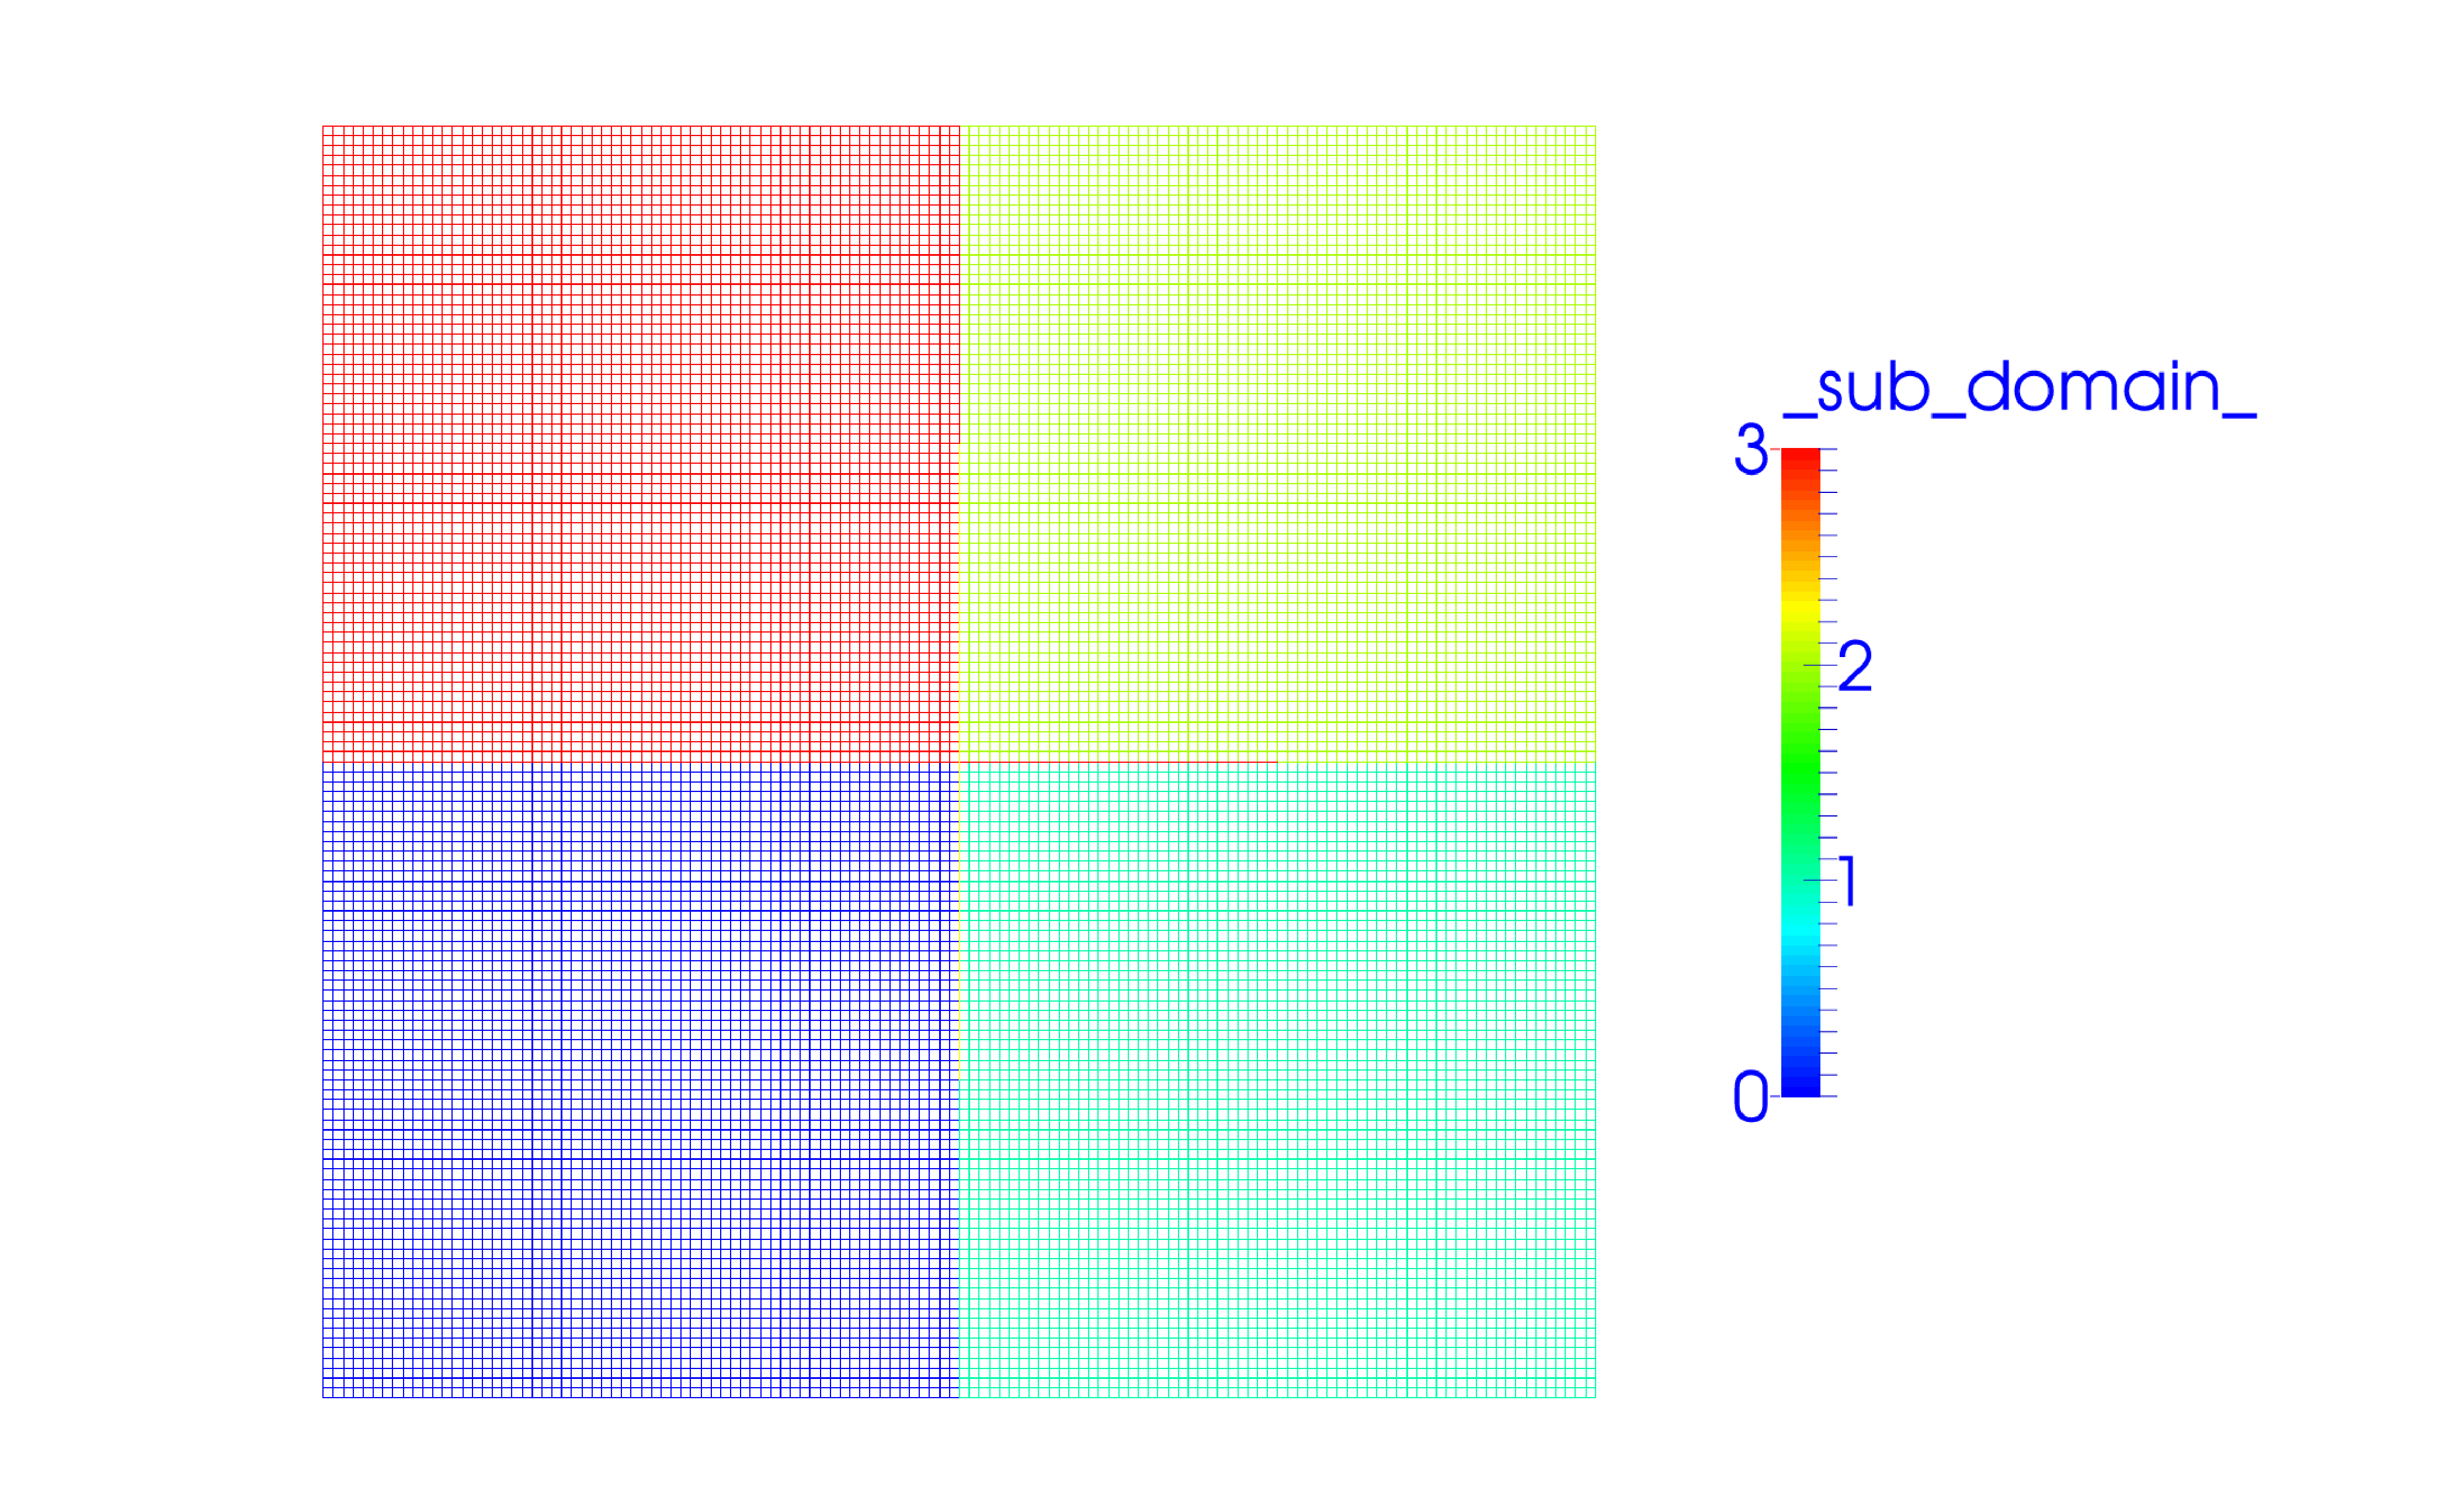
\includegraphics[width=0.95\textwidth]{fig/mesh.pdf}
  \caption{Refined 2-dimensional mesh used for the example.}
  \label{fig:mesh}
\end{figure}

\begin{figure}
\centering
	\subfloat[PC mode 0]{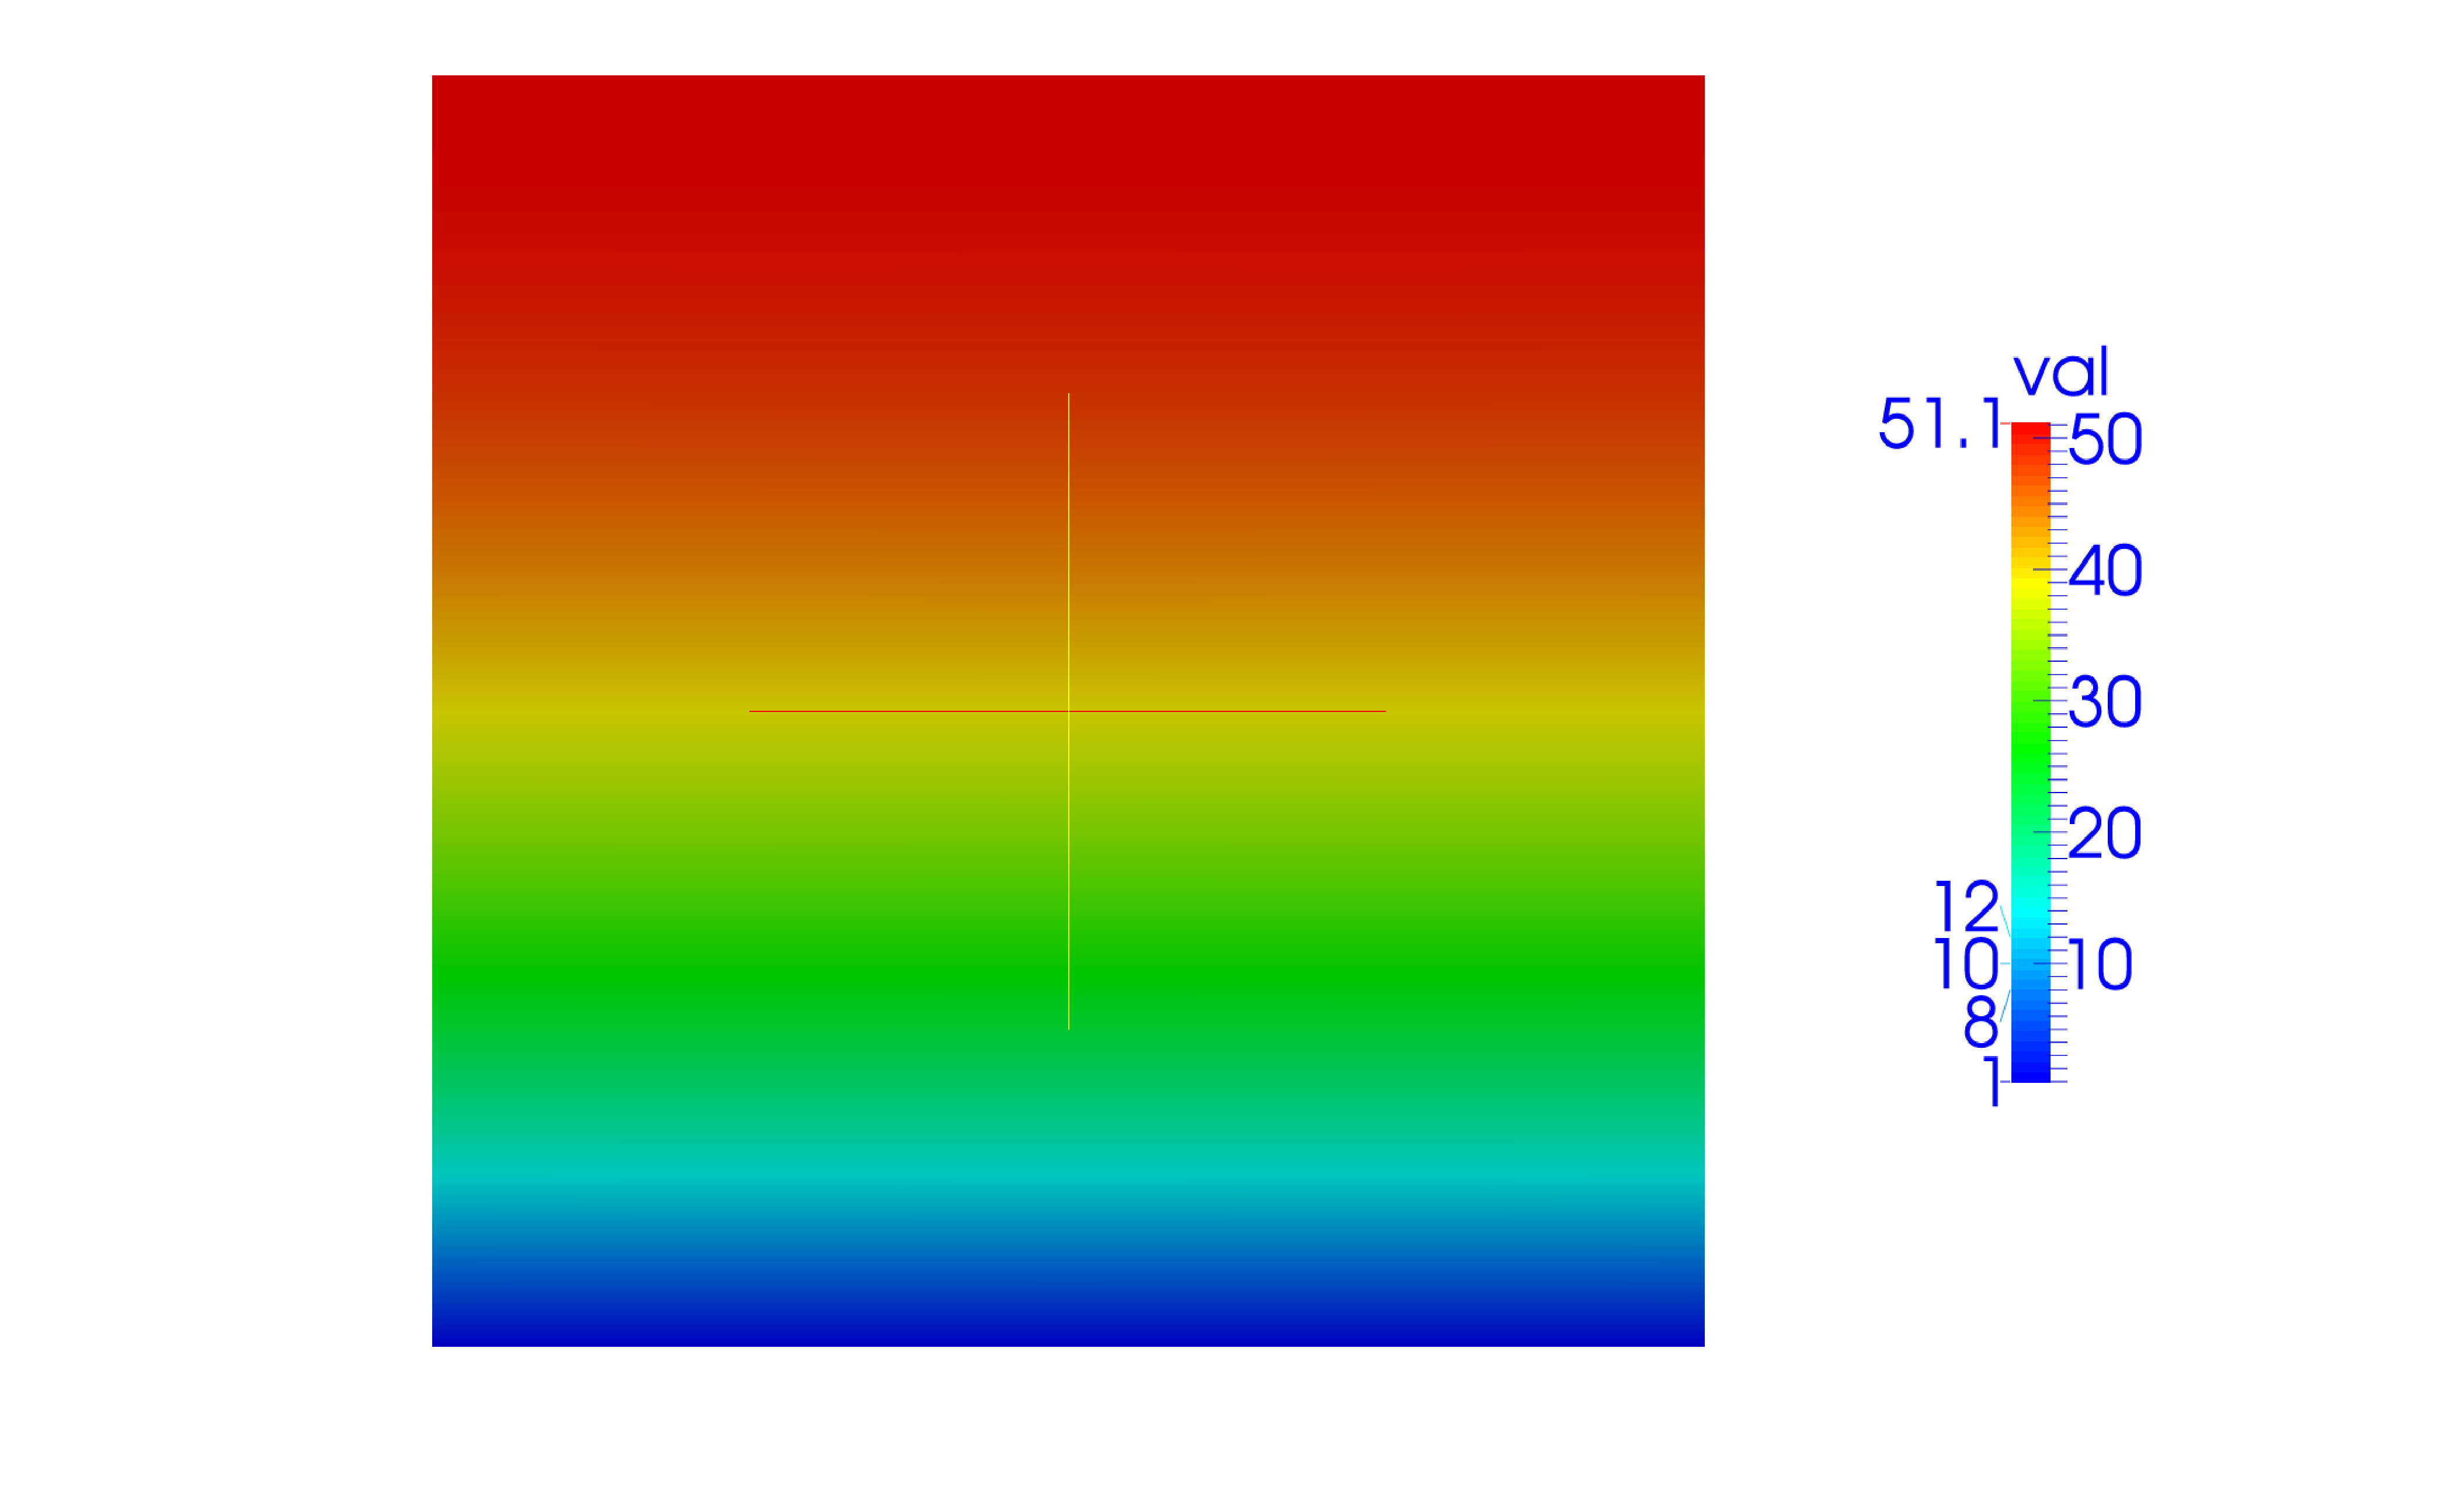
\includegraphics[width = 0.48\textwidth]{fig/mode0.pdf}} 
	\subfloat[PC mode 1]{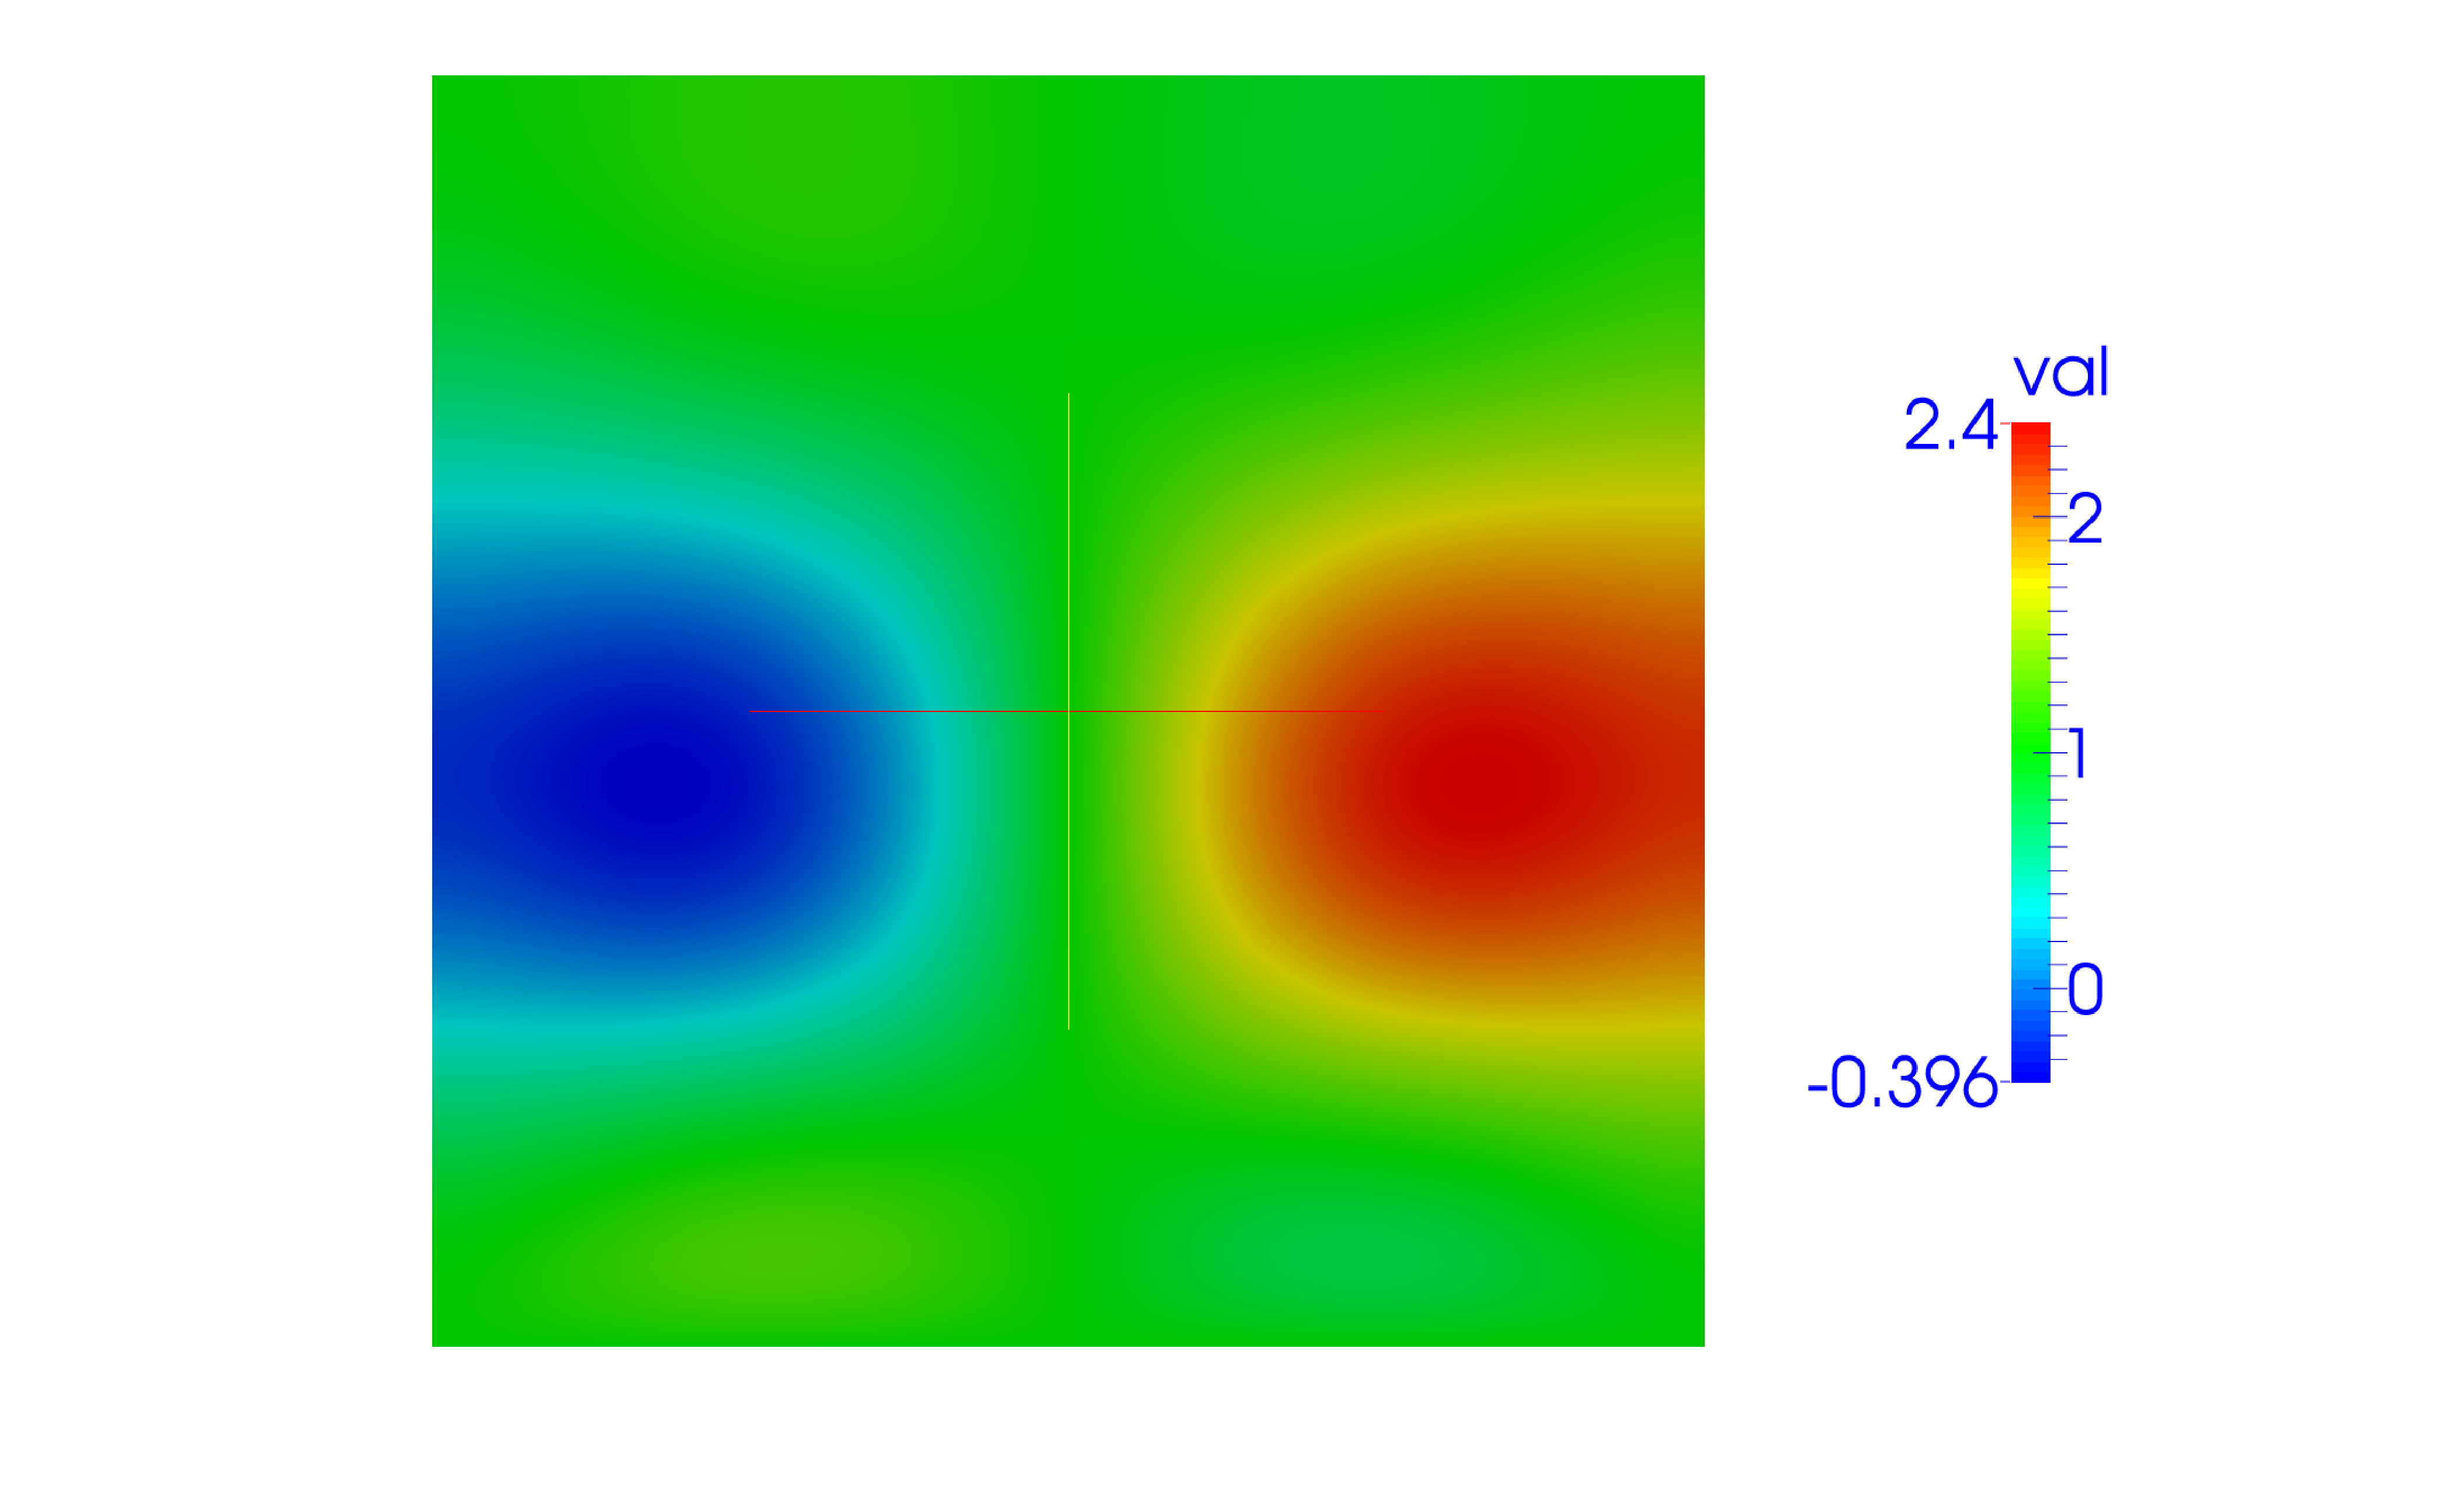
\includegraphics[width = 0.48\textwidth]{fig/mode1.pdf}}\\
	\subfloat[PC mode 2]{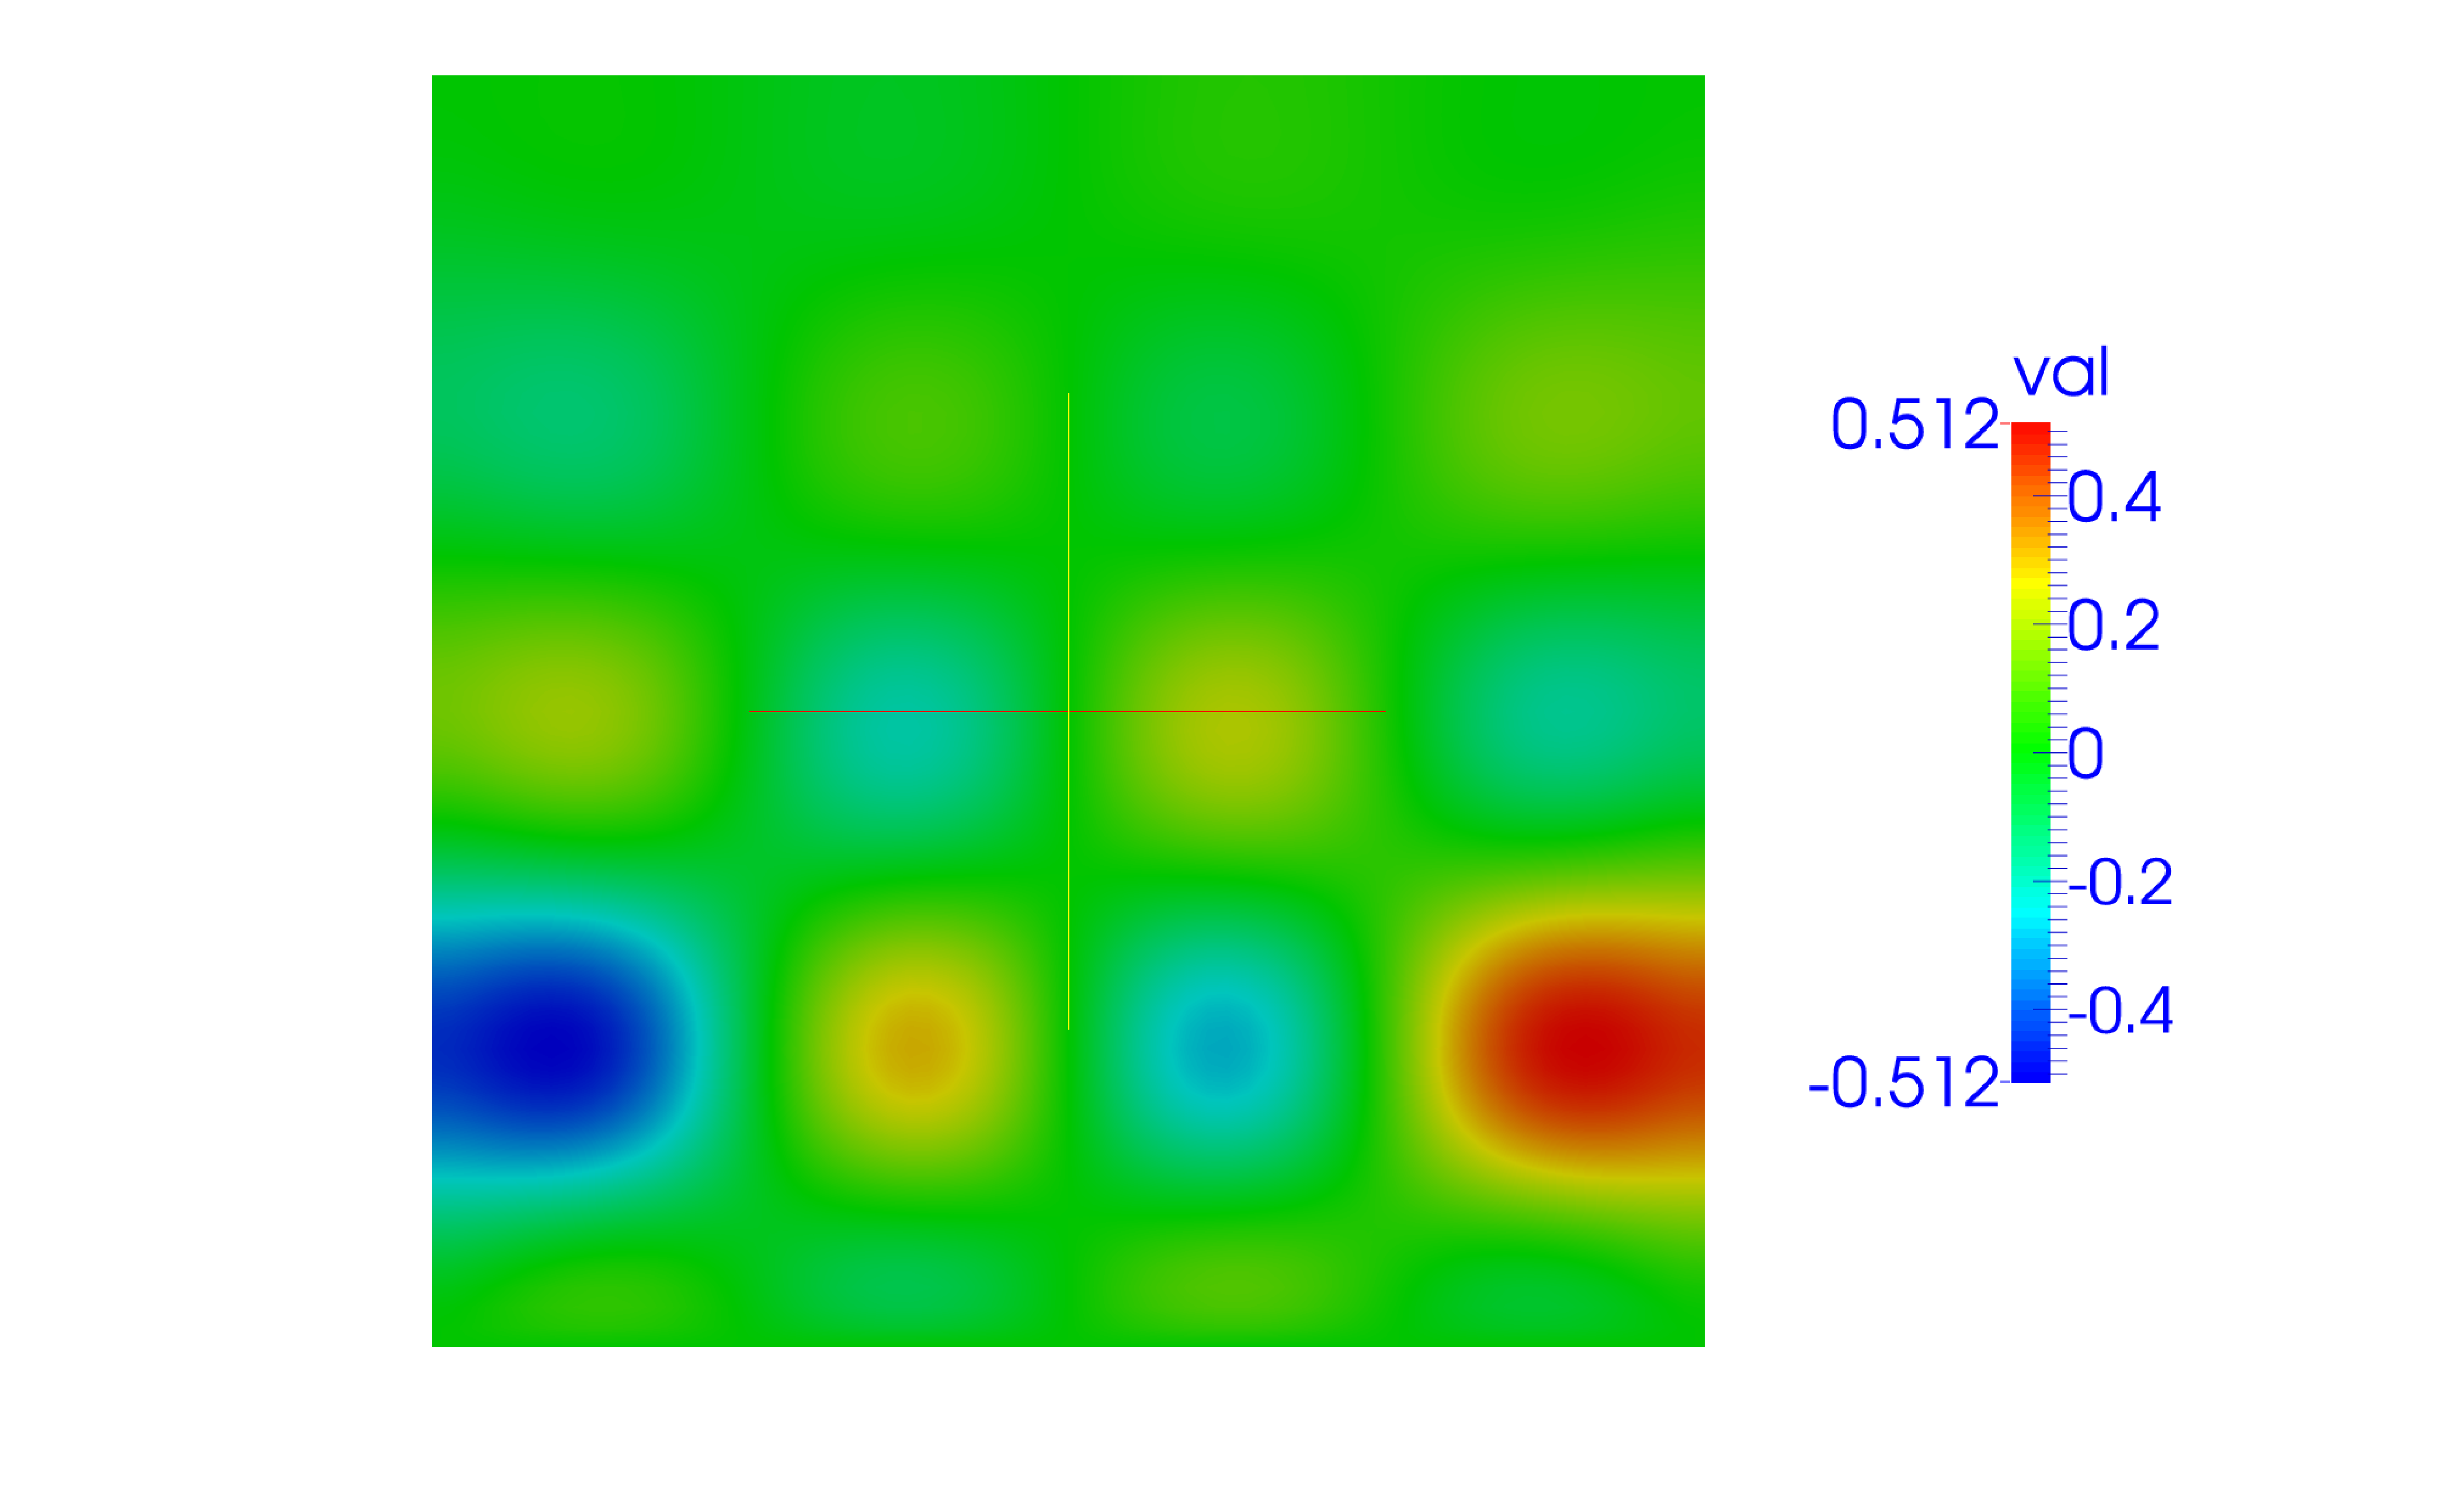
\includegraphics[width = 0.48\textwidth]{fig/mode2.pdf}}
	\subfloat[PC mode 3]{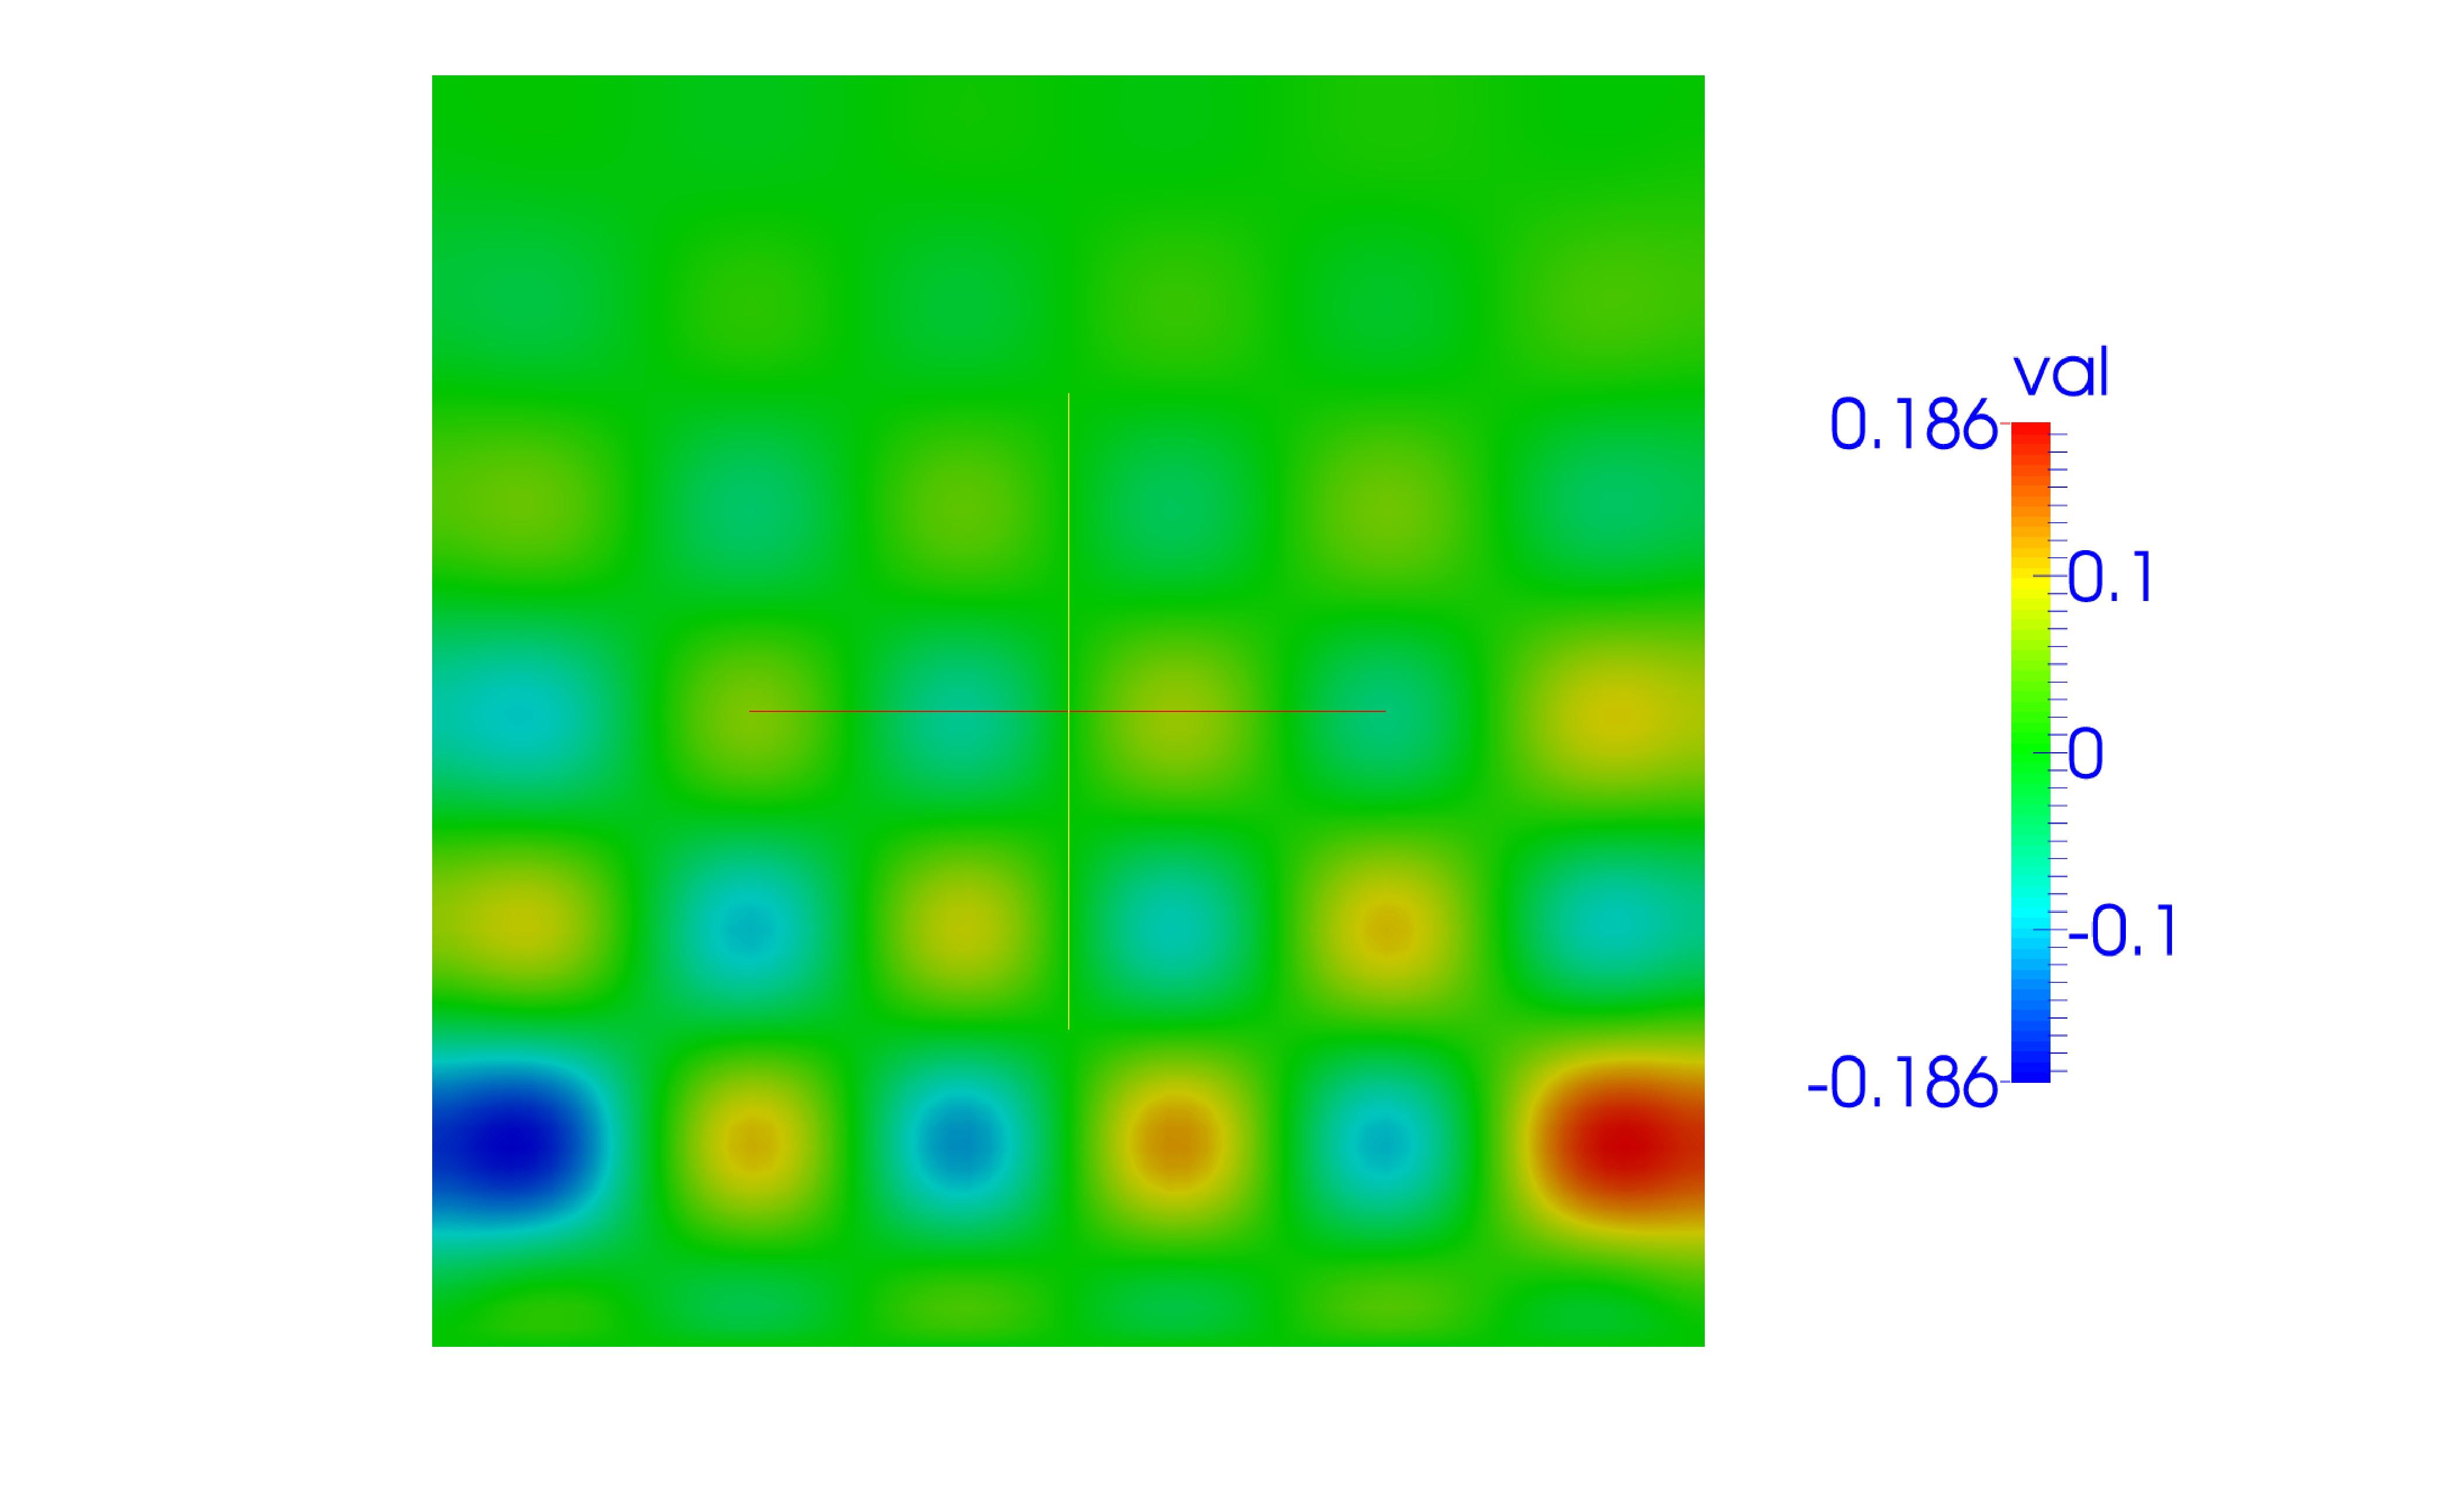
\includegraphics[width = 0.48\textwidth]{fig/mode3.pdf}} 
\caption{The first 4 Polynomial Chaos (PC) mode results.}
\label{fig:modes}
\end{figure}

The Figure \ref{fig:mesh} shows the discrete mesh and how it is distributed over four processors, and the Figure \ref{fig:modes} presents selected results of the first 4 modes (over 20). Moreover, the result of mode 0 corresponds to the mean value of the stochastic poisson system.



\pagebreak


%% ++++++++++++++++++++++++++++++++++++++++++
\pagebreak
\phantomsection
\addcontentsline{toc}{section}{\bibname}


\newpage
\appendix
\bibliography{tut_stochastic_poisson}
\bibliographystyle{plain}


%% ++++++++++++++++++++++++++++++++++++++++++
%% Index
%% ++++++++++++++++++++++++++++++++++++++++++
\cleardoublepage
\phantomsection
\addcontentsline{toc}{section}{Index}
\printindex            % Index, Stichwortverzeichnis
\end{document}
%% end of file
